\documentclass[a4paper,12pt]{article}

% ========================================================================
% Packages
% ========================================================================
\usepackage[margin=2cm]{geometry}
\usepackage{tikz}
\usepackage{amsmath}
\usepackage{amssymb}
\usepackage{graphicx}
\usepackage{float}

% TikZ Libraries
\usetikzlibrary{
    arrows.meta,
    positioning,
    calc,
    shapes.geometric,
    fit,
    decorations.markings,
    patterns
}

% ========================================================================
% Shared TikZ Style Definitions
% ========================================================================
\tikzset{
    % --- Sub-block (abstracted entity shown as rectangle) ---
    block/.style = {
        rectangle, draw, very thick,
        minimum width=3.5cm, minimum height=1.8cm,
        font=\sffamily\small, align=center,
        text width=3cm
    },
    % --- Wider block for top-level stages ---
    wide block/.style = {
        block, minimum width=5cm, text width=4.5cm
    },
    % --- Small utility block (delay, mux, ROM) ---
    small block/.style = {
        rectangle, draw, thick,
        minimum width=2cm, minimum height=1cm,
        font=\sffamily\footnotesize, align=center
    },
    % --- Arithmetic operator circle ---
    operator/.style = {
        circle, draw, very thick,
        minimum size=9mm,
        font=\sffamily\large,
        inner sep=0pt, fill=white
    },
    % --- Wire junction dot ---
    dot/.style = {
        circle, fill=black,
        minimum size=3pt, inner sep=0pt
    },
    % --- Port label (bold, input/output names) ---
    port/.style = {
        font=\sffamily\bfseries\small
    },
    % --- Signal label on wire ---
    signal/.style = {
        font=\sffamily\footnotesize,
        fill=white, inner sep=1pt
    },
    % --- Bus width slash annotation ---
    bus/.style = {
        font=\sffamily\scriptsize
    },
    % --- Dashed enclosure (entity boundary or FSM) ---
    entity border/.style = {
        rectangle, draw, dashed, thick,
        rounded corners=3pt, inner sep=8pt
    },
    % --- Pipeline stage separator ---
    stage sep/.style = {
        dashed, thin, black!50
    },
    % --- Register box (D flip-flop) ---
    register/.style = {
        rectangle, draw, thick,
        minimum width=1.0cm, minimum height=0.8cm,
        font=\sffamily\footnotesize, align=center
    },
    % --- Data flow arrow ---
    data arrow/.style = {
        -Stealth, thick
    },
    % --- Control signal arrow ---
    ctrl arrow/.style = {
        -Stealth, thin, dashed
    },
    % --- Constant/generic input label ---
    const/.style = {
        font=\sffamily\itshape\footnotesize
    },
    % --- Annotation text ---
    annotation/.style = {
        font=\sffamily\small,
        align=left
    },
    % --- General thick arrow (default for connections) ---
    >=Stealth,
    thick,
    font=\sffamily
}

% ========================================================================
% Bus slash macro
% ========================================================================
\newcommand{\busmark}[1]{%
    \tikz[baseline=-0.5ex]{
        \draw[thick] (-0.15,-0.15) -- (0.15,0.15);
        \node[font=\sffamily\scriptsize, above left=-1pt] {#1};
    }%
}

% ========================================================================
% Document
% ========================================================================
\begin{document}

\begin{center}
    {\LARGE\sffamily\bfseries Block Diagrams: Neural Network DPD in VHDL}\\[3mm]
    {\large\sffamily CMEMP Model -- Fixed-Point Q16.16 Implementation}
\end{center}

\vspace{5mm}

% ---- Top-Level ----
\section{System Architecture}
\begin{figure}[H]
\centering
\resizebox{\textwidth}{!}{%
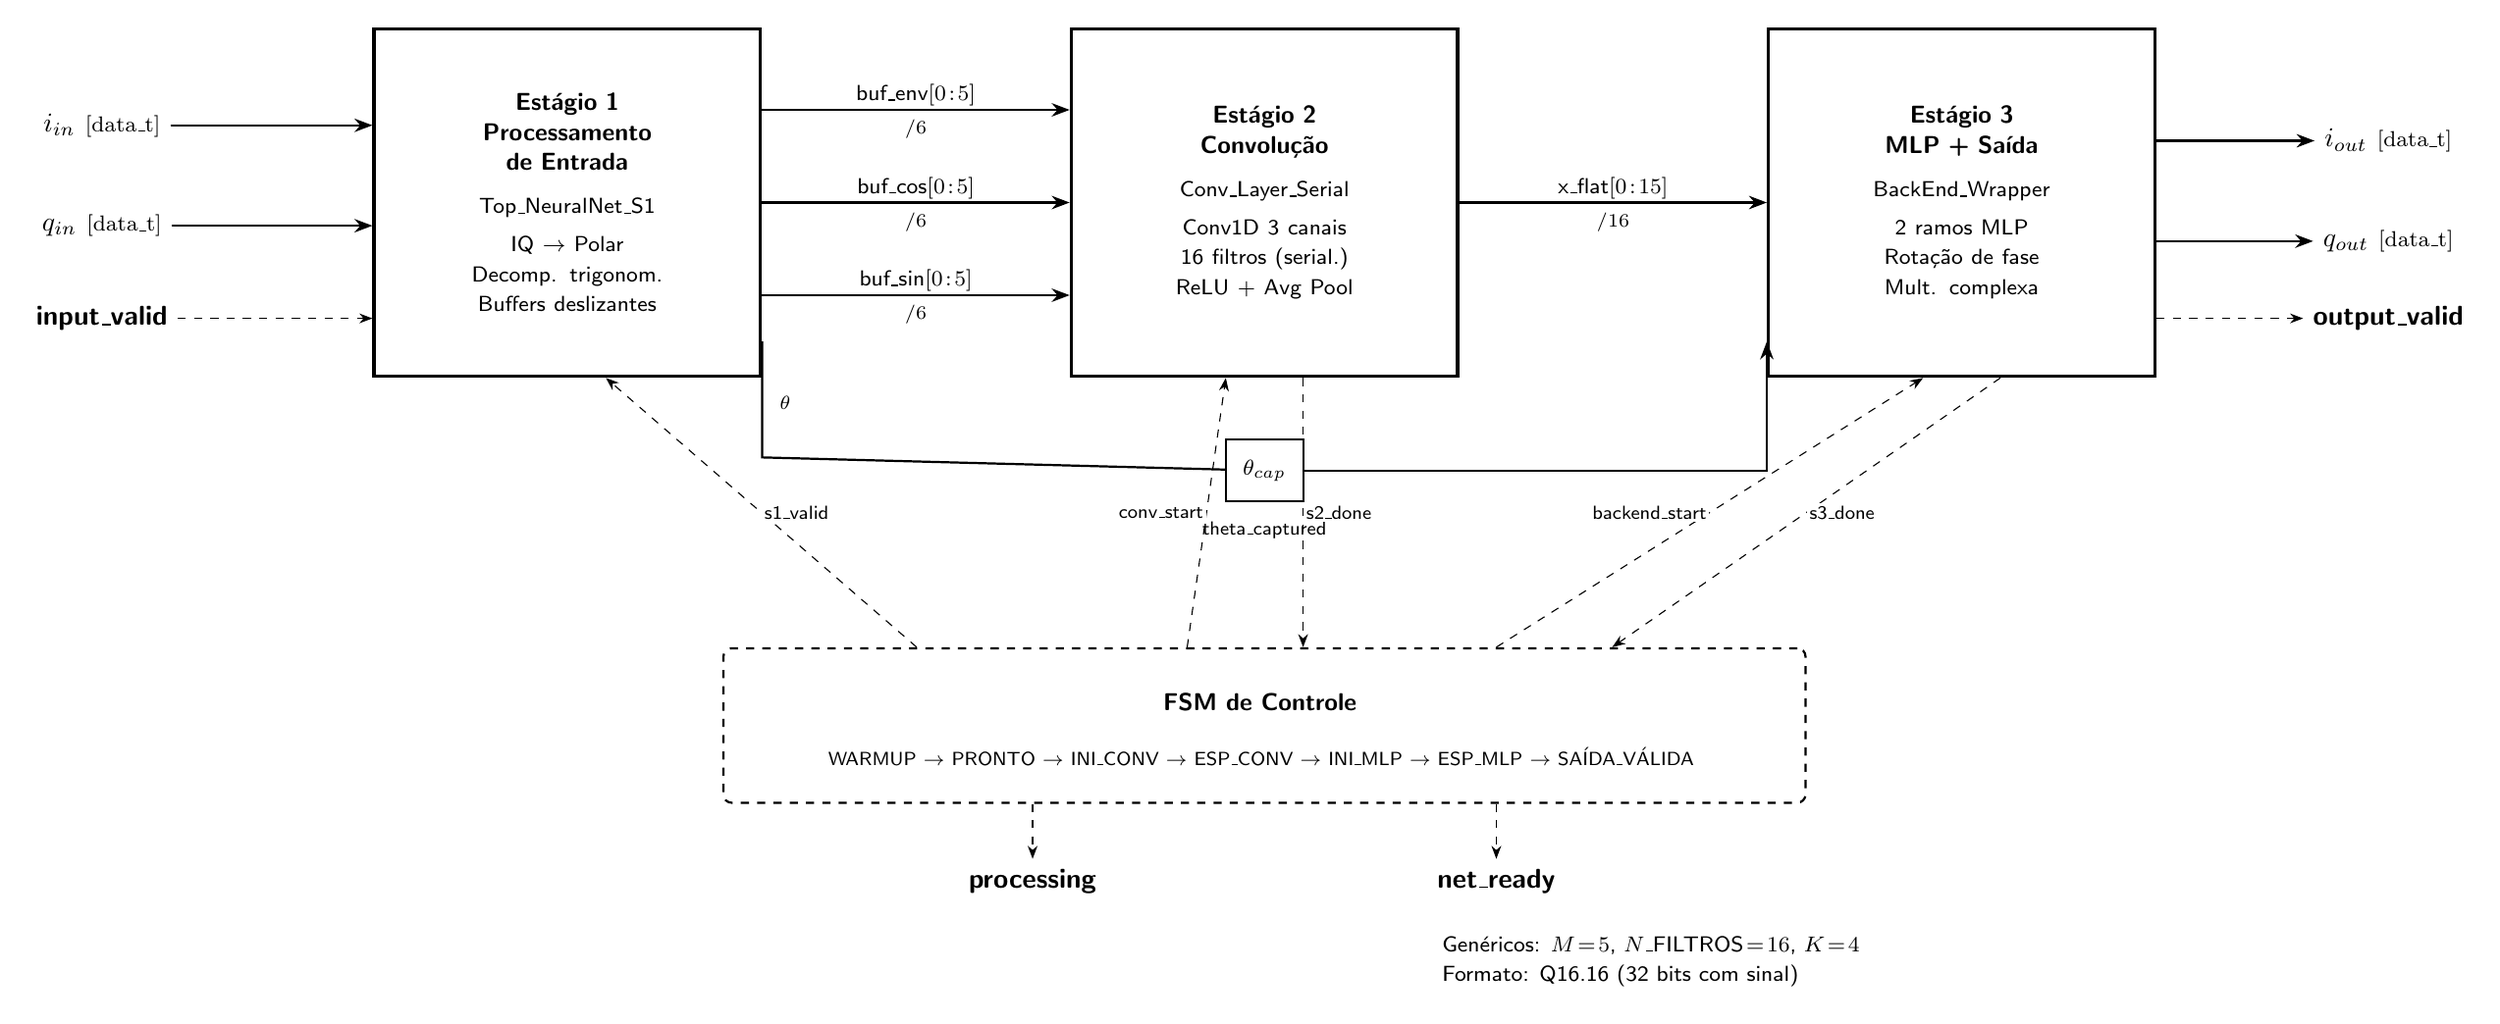
\begin{tikzpicture}[
    node distance=1.5cm and 2.5cm,
    >=Stealth, thick, font=\sffamily
]

\tikzset{
    io_node/.style={font=\sffamily\bfseries},
    dot/.style={circle, fill=black, inner sep=0pt, minimum size=4pt}
}

% ---------------------------------------------------------
% Tres estagios de pipeline
% ---------------------------------------------------------
\node[wide block, minimum height=4.5cm, text width=4.0cm] (S1) at (0, 0) {%
    \textbf{Est\'{a}gio 1}\\
    \textbf{Processamento}\\
    \textbf{de Entrada}\\[5pt]
    {\footnotesize Top\_NeuralNet\_S1}\\[3pt]
    {\footnotesize IQ $\rightarrow$ Polar}\\
    {\footnotesize Decomp. trigonom.}\\
    {\footnotesize Buffers deslizantes}
};

\node[wide block, minimum height=4.5cm, text width=4.0cm] (S2) at ($(S1.east) + (6.5, 0)$) {%
    \textbf{Est\'{a}gio 2}\\
    \textbf{Convolu\c{c}\~{a}o}\\[5pt]
    {\footnotesize Conv\_Layer\_Serial}\\[3pt]
    {\footnotesize Conv1D 3 canais}\\
    {\footnotesize 16 filtros (serial.)}\\
    {\footnotesize ReLU + Avg Pool}
};

\node[wide block, minimum height=4.5cm, text width=4.0cm] (S3) at ($(S2.east) + (6.5, 0)$) {%
    \textbf{Est\'{a}gio 3}\\
    \textbf{MLP + Sa\'{i}da}\\[5pt]
    {\footnotesize BackEnd\_Wrapper}\\[3pt]
    {\footnotesize 2 ramos MLP}\\
    {\footnotesize Rota\c{c}\~{a}o de fase}\\
    {\footnotesize Mult. complexa}
};

% ---------------------------------------------------------
% Portas de entrada (extremo esquerdo)
% ---------------------------------------------------------
\node[io_node] (Iin) at ($(S1.west) + (-3.5, 1.0)$) {$i_{in}$ \normalfont\footnotesize [data\_t]};
\node[io_node] (Qin) at ($(S1.west) + (-3.5, -0.3)$) {$q_{in}$ \normalfont\footnotesize [data\_t]};
\node[io_node] (Vin) at ($(S1.west) + (-3.5, -1.5)$) {input\_valid};

\draw[data arrow] (Iin) -- ($(S1.west) + (0, 1.0)$);
\draw[data arrow] (Qin) -- ($(S1.west) + (0, -0.3)$);
\draw[ctrl arrow] (Vin) -- ($(S1.west) + (0, -1.5)$);

% ---------------------------------------------------------
% S1 -> S2: barramentos de buffer
% ---------------------------------------------------------
\draw[data arrow] ($(S1.east) + (0, 1.2)$) -- ($(S2.west) + (0, 1.2)$)
    node[signal, midway, above] {buf\_env$[0\!:\!5]$}
    node[bus, midway, below] {$/6$};

\draw[data arrow] ($(S1.east) + (0, 0.0)$) -- ($(S2.west) + (0, 0.0)$)
    node[signal, midway, above] {buf\_cos$[0\!:\!5]$}
    node[bus, midway, below] {$/6$};

\draw[data arrow] ($(S1.east) + (0, -1.2)$) -- ($(S2.west) + (0, -1.2)$)
    node[signal, midway, above] {buf\_sin$[0\!:\!5]$}
    node[bus, midway, below] {$/6$};

% ---------------------------------------------------------
% S1 -> S3: bypass de theta (abaixo do S2)
% ---------------------------------------------------------
\coordinate (thetaStart) at ($(S1.east) + (0, -1.8)$);
\coordinate (thetaEnd) at ($(S3.west) + (0, -1.8)$);
\coordinate (thetaBelow) at ($(S2.south) + (0, -1.2)$);

\draw[data arrow] (thetaStart) -- ++(0, -1.5) -- (thetaBelow);
\node[register, fill=white] (ThetaReg) at (thetaBelow) {$\theta_{cap}$};
\node[signal, below=0.2cm of ThetaReg] {\scriptsize theta\_captured};
\draw[data arrow] (ThetaReg.east) -| (thetaEnd);
\node[signal] at ($(thetaStart) + (0.3, -0.8)$) {\scriptsize $\theta$};

% ---------------------------------------------------------
% S2 -> S3: vetor de features
% ---------------------------------------------------------
\draw[data arrow] ($(S2.east) + (0, 0.0)$) -- ($(S3.west) + (0, 0.0)$)
    node[signal, midway, above] {x\_flat$[0\!:\!15]$}
    node[bus, midway, below] {$/16$};

% ---------------------------------------------------------
% Portas de saida (extremo direito)
% ---------------------------------------------------------
\node[io_node] (Iout) at ($(S3.east) + (3.0, 0.8)$) {$i_{out}$ \normalfont\footnotesize [data\_t]};
\node[io_node] (Qout) at ($(S3.east) + (3.0, -0.5)$) {$q_{out}$ \normalfont\footnotesize [data\_t]};
\node[io_node] (Vout) at ($(S3.east) + (3.0, -1.5)$) {output\_valid};

\draw[data arrow] ($(S3.east) + (0, 0.8)$) -- (Iout);
\draw[data arrow] ($(S3.east) + (0, -0.5)$) -- (Qout);
\draw[ctrl arrow] ($(S3.east) + (0, -1.5)$) -- (Vout);

% ---------------------------------------------------------
% FSM de Controle (baixo)
% ---------------------------------------------------------
\node[entity border, minimum width=14.0cm, minimum height=2.0cm] (FSM) at ($(S2.south) + (0, -4.5)$) {};
\node[font=\sffamily\small\bfseries, align=center] at ($(FSM.center) + (0, 0.3)$) {%
    FSM de Controle
};
\node[font=\sffamily\scriptsize, align=center] at ($(FSM.center) + (0, -0.4)$) {%
    WARMUP $\rightarrow$ PRONTO $\rightarrow$ INI\_CONV $\rightarrow$ ESP\_CONV $\rightarrow$ INI\_MLP $\rightarrow$ ESP\_MLP $\rightarrow$ SA\'{I}DA\_V\'{A}LIDA
};

% Sinais de controle FSM <-> Estagios
\draw[ctrl arrow] ($(FSM.north) + (-4.5, 0)$) -- ($(S1.south) + (0.5, 0)$)
    node[signal, midway, right] {\scriptsize s1\_valid};

\draw[ctrl arrow] ($(FSM.north) + (-1.0, 0)$) -- ($(S2.south) + (-0.5, 0)$)
    node[signal, midway, left] {\scriptsize conv\_start};

\draw[ctrl arrow] ($(S2.south) + (0.5, 0)$) -- ($(FSM.north) + (0.5, 0)$)
    node[signal, midway, right] {\scriptsize s2\_done};

\draw[ctrl arrow] ($(FSM.north) + (3.0, 0)$) -- ($(S3.south) + (-0.5, 0)$)
    node[signal, midway, left] {\scriptsize backend\_start};

\draw[ctrl arrow] ($(S3.south) + (0.5, 0)$) -- ($(FSM.north) + (4.5, 0)$)
    node[signal, midway, right] {\scriptsize s3\_done};

% Saidas de status da FSM
\node[io_node] (Proc) at ($(FSM.south) + (-3.0, -1.0)$) {processing};
\node[io_node] (Ready) at ($(FSM.south) + (3.0, -1.0)$) {net\_ready};

\draw[ctrl arrow] ($(FSM.south) + (-3.0, 0)$) -- (Proc);
\draw[ctrl arrow] ($(FSM.south) + (3.0, 0)$) -- (Ready);

% ---------------------------------------------------------
% Anotacao de generics
% ---------------------------------------------------------
\node[annotation, below=0.3cm of Ready, xshift=2cm] {%
    {\footnotesize Gen\'{e}ricos: $M\!=\!5$,\ $N\_\text{FILTROS}\!=\!16$,\ $K\!=\!4$}\\
    {\footnotesize Formato: Q16.16 (32~bits com sinal)}
};

\end{tikzpicture}%
}

\vspace{3mm}
\noindent\textit{Pipeline de tr\^{e}s est\'{a}gios controlado por uma FSM central. O Est\'{a}gio~1 opera continuamente; os Est\'{a}gios~2 e~3 s\~{a}o ativados sequencialmente ap\'{o}s \textit{warmup} ($M\!=\!5$ amostras). A fase $\theta$ realiza \textit{bypass} do Est\'{a}gio~2 via registrador de captura.}

\caption{NeuralNet\_Complete -- arquitetura geral do sistema de pr\'{e}-distor\c{c}\~{a}o digital baseado em rede neural.}
\label{fig:neuralnet_complete}
\end{figure}


% ---- Stage 1 ----
\section{Stage 1: Input Processing}
\begin{figure}[H]
\centering
\resizebox{\textwidth}{!}{%
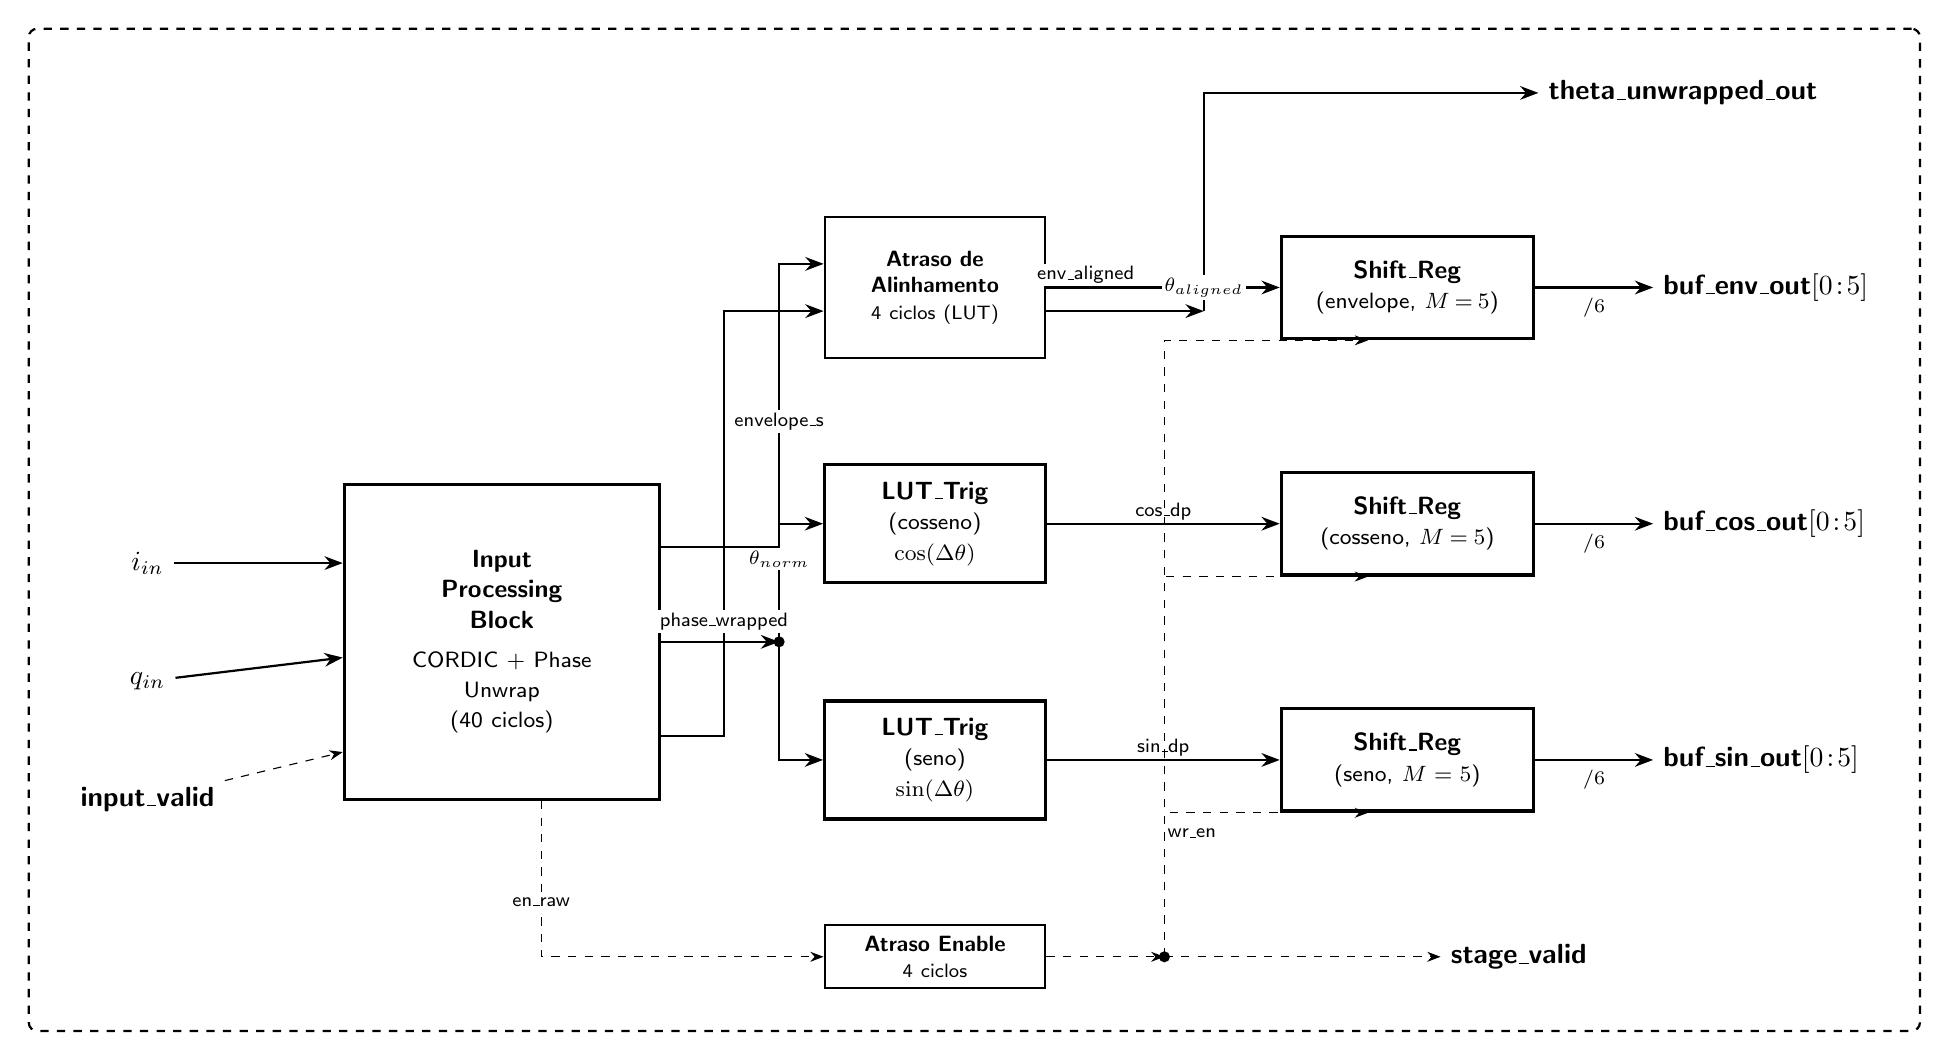
\begin{tikzpicture}[
    node distance=1.2cm and 1.8cm,
    >=Stealth, thick, font=\sffamily
]

\tikzset{
    io_node/.style={font=\sffamily\bfseries},
    dot/.style={circle, fill=black, inner sep=0pt, minimum size=4pt}
}

% ---------------------------------------------------------
% Bloco de Processamento de Entrada (esquerda)
% ---------------------------------------------------------
\node[block, minimum width=4.0cm, minimum height=4.0cm, text width=3.5cm] (IPB) at (0, 0) {%
    \textbf{Input}\\
    \textbf{Processing}\\
    \textbf{Block}\\[3pt]
    {\footnotesize CORDIC + Phase}\\
    {\footnotesize Unwrap}\\
    {\footnotesize (40 ciclos)}
};

% ---------------------------------------------------------
% Entradas (extremo esquerdo)
% ---------------------------------------------------------
\node[io_node] (Iin) at (-4.5, 1.0) {$i_{in}$};
\node[io_node] (Qin) at (-4.5, -0.5) {$q_{in}$};
\node[io_node] (Vin) at (-4.5, -2.0) {input\_valid};

\draw[data arrow] (Iin) -- ($(IPB.west) + (0, 1.0)$);
\draw[data arrow] (Qin) -- ($(IPB.west) + (0, -0.2)$);
\draw[ctrl arrow] (Vin) -- ($(IPB.west) + (0, -1.4)$);

% ---------------------------------------------------------
% Sa\'idas do IPB
% ---------------------------------------------------------
% envelope_s (topo direito do IPB)
\coordinate (envOut) at ($(IPB.east) + (0, 1.2)$);
% theta_norm (meio direito do IPB)
\coordinate (thetaNormOut) at ($(IPB.east) + (0, 0.0)$);
% phase_wrapped (baixo direito do IPB)
\coordinate (phaseWOut) at ($(IPB.east) + (0, -1.2)$);
% buffers_enable_raw (base do IPB)
\coordinate (enRawOut) at ($(IPB.south) + (0.5, 0)$);

% ---------------------------------------------------------
% LUTs trigonometricas (secao central)
% ---------------------------------------------------------
\node[block, minimum width=2.8cm, minimum height=1.5cm, text width=2.4cm] (LUT_C) at (5.5, 1.5) {%
    \textbf{LUT\_Trig}\\
    {\footnotesize (cosseno)}\\
    {\footnotesize $\cos(\Delta\theta)$}
};

\node[block, minimum width=2.8cm, minimum height=1.5cm, text width=2.4cm] (LUT_S) at (5.5, -1.5) {%
    \textbf{LUT\_Trig}\\
    {\footnotesize (seno)}\\
    {\footnotesize $\sin(\Delta\theta)$}
};

% theta_norm bifurca para ambas LUTs
\draw[data arrow] (thetaNormOut) -- ++(1.5, 0) coordinate (thetaFork);
\node[dot] at (thetaFork) {};
\draw[data arrow] (thetaFork) |- (LUT_C.west)
    node[signal, pos=0.3, above] {\scriptsize $\theta_{norm}$};
\draw[data arrow] (thetaFork) |- (LUT_S.west);

% ---------------------------------------------------------
% Bloco de Atraso de Alinhamento (envelope + theta)
% ---------------------------------------------------------
\node[small block, minimum width=2.8cm, minimum height=1.8cm, text width=2.4cm] (Delay) at (5.5, 4.5) {%
    \textbf{Atraso de}\\
    \textbf{Alinhamento}\\
    {\scriptsize 4 ciclos (LUT)}
};

% envelope_s -> Atraso
\draw[data arrow] (envOut) -- ++(1.5, 0) |- ($(Delay.west) + (0, 0.3)$)
    node[signal, pos=0.2, above] {\scriptsize envelope\_s};

% phase_wrapped -> Atraso (caminho theta)
\draw[data arrow] (phaseWOut) -- ++(0.8, 0) |- ($(Delay.west) + (0, -0.3)$)
    node[signal, pos=0.15, below] {\scriptsize phase\_wrapped};

% ---------------------------------------------------------
% Atraso do Enable
% ---------------------------------------------------------
\node[small block, minimum width=2.8cm, minimum height=0.8cm, text width=2.4cm] (EnDelay) at (5.5, -4.0) {%
    \textbf{Atraso Enable}\\
    {\scriptsize 4 ciclos}
};
\draw[ctrl arrow] (enRawOut) |- (EnDelay.west)
    node[signal, pos=0.3, below] {\scriptsize en\_raw};

% ---------------------------------------------------------
% Registradores de Deslocamento (secao direita)
% ---------------------------------------------------------
\node[block, minimum width=3.2cm, minimum height=1.3cm, text width=2.8cm] (SR_E) at (11.5, 4.5) {%
    \textbf{Shift\_Reg}\\
    {\footnotesize (envelope, $M\!=\!5$)}
};

\node[block, minimum width=3.2cm, minimum height=1.3cm, text width=2.8cm] (SR_C) at (11.5, 1.5) {%
    \textbf{Shift\_Reg}\\
    {\footnotesize (cosseno, $M\!=\!5$)}
};

\node[block, minimum width=3.2cm, minimum height=1.3cm, text width=2.8cm] (SR_S) at (11.5, -1.5) {%
    \textbf{Shift\_Reg}\\
    {\footnotesize (seno, $M\!=\!5$)}
};

% Atraso -> Shift_Reg (envelope)
\draw[data arrow] (Delay.east) -- ++(0.5, 0) |- (SR_E.west)
    node[signal, pos=0.4, above] {\scriptsize env\_aligned};

% LUT_C -> Shift_Reg (cos)
\draw[data arrow] (LUT_C.east) -- (SR_C.west)
    node[signal, midway, above] {\scriptsize cos\_dp};

% LUT_S -> Shift_Reg (sin)
\draw[data arrow] (LUT_S.east) -- (SR_S.west)
    node[signal, midway, above] {\scriptsize sin\_dp};

% Distribuicao do enable
\coordinate (enAligned) at ($(EnDelay.east) + (1.5, 0)$);
\draw[ctrl arrow] (EnDelay.east) -- (enAligned);
\node[dot] at (enAligned) {};
\draw[ctrl arrow] (enAligned) |- ($(SR_E.south) + (-0.5, 0)$)
    node[signal, pos=0.1, right] {\scriptsize wr\_en};
\draw[ctrl arrow] (enAligned) |- ($(SR_C.south) + (-0.5, 0)$);
\draw[ctrl arrow] (enAligned) |- ($(SR_S.south) + (-0.5, 0)$);

% ---------------------------------------------------------
% Saidas (extremo direito)
% ---------------------------------------------------------
\node[io_node, right=1.5cm of SR_E] (OutE) {buf\_env\_out$[0\!:\!5]$};
\node[io_node, right=1.5cm of SR_C] (OutC) {buf\_cos\_out$[0\!:\!5]$};
\node[io_node, right=1.5cm of SR_S] (OutS) {buf\_sin\_out$[0\!:\!5]$};

\draw[data arrow] (SR_E.east) -- (OutE) node[bus, midway, below] {$/6$};
\draw[data arrow] (SR_C.east) -- (OutC) node[bus, midway, below] {$/6$};
\draw[data arrow] (SR_S.east) -- (OutS) node[bus, midway, below] {$/6$};

% ---------------------------------------------------------
% theta_unwrapped_out (CORRIGIDO: acima de buf_env, sem sobreposicao)
% ---------------------------------------------------------
% Posicionado bem acima da linha do SR_E para evitar colisao visual
\node[io_node] (OutTheta) at ($(SR_E.north) + (3.5, 1.8)$) {theta\_unwrapped\_out};

% Fio: do lado leste do Delay, sobe ate a saida de theta
\draw[data arrow] ($(Delay.east) + (0, -0.3)$) -- ++(2.0, 0) coordinate (ThetaMid);
\draw[data arrow] (ThetaMid) -- ($(ThetaMid |- OutTheta)$) -- (OutTheta);
\node[signal] at ($(ThetaMid) + (0, 0.3)$) {\scriptsize $\theta_{aligned}$};

% ---------------------------------------------------------
% stage_valid
% ---------------------------------------------------------
\node[io_node] (OutValid) at ($(enAligned) + (4.5, 0)$) {stage\_valid};
\draw[ctrl arrow] (enAligned) -- ++(0.5, 0) |- (OutValid);

% ---------------------------------------------------------
% Borda da entidade
% ---------------------------------------------------------
\node[entity border, fit=(Iin)(Vin)(OutE)(OutS)(OutTheta)(OutValid)(Delay)(EnDelay), inner sep=15pt] {};

\end{tikzpicture}%
}

\vspace{3mm}
\noindent\textit{Lat\^{e}ncia das LUTs $= 4$ ciclos. O atraso de alinhamento garante sincronismo do envelope e de $\theta$ com as sa\'{i}das das LUTs. Todos os registradores de deslocamento avancam simultaneamente com \textsf{wr\_en}.}

\caption{Top\_NeuralNet\_S1 -- Est\'{a}gio 1: convers\~{a}o IQ$\,\rightarrow\,$polar, decomposi\c{c}\~{a}o trigonom\'{e}trica e buffers deslizantes.}
\label{fig:top_neuralnet_s1}
\end{figure}


\subsection{Input Processing Block}
\begin{figure}[H]
\centering
\resizebox{\textwidth}{!}{%
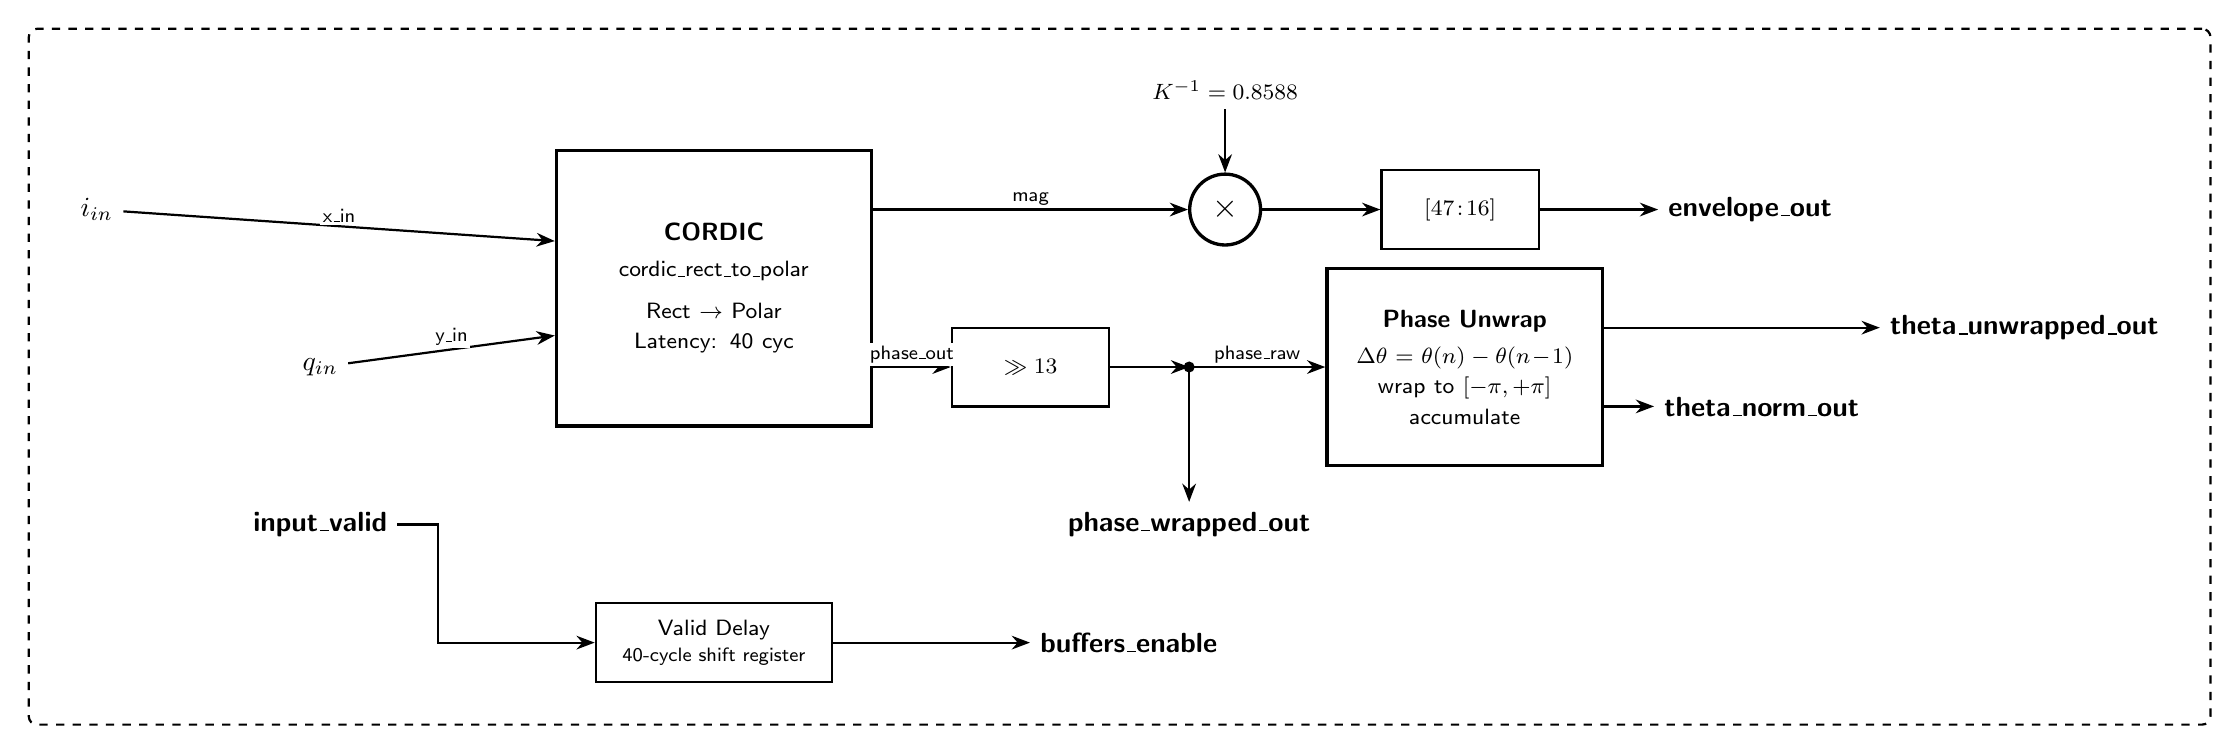
\begin{tikzpicture}[
    node distance=1.2cm and 2.0cm,
    >=Stealth, thick, font=\sffamily
]

% ---------------------------------------------------------
% Styles
% ---------------------------------------------------------
\tikzset{
    op_node/.style={
        circle, draw=black, very thick, minimum size=0.9cm, fill=white,
        font=\sffamily\large
    },
    io_node/.style={font=\sffamily\bfseries},
    dot/.style={circle, fill=black, inner sep=0pt, minimum size=4pt}
}

% ---------------------------------------------------------
% CORDIC block (large)
% ---------------------------------------------------------
\node[block, minimum width=4.0cm, minimum height=3.5cm, text width=3.5cm] (CORDIC) at (0, 0) {%
    \textbf{CORDIC}\\[2pt]
    \textsf{\footnotesize cordic\_rect\_to\_polar}\\[4pt]
    {\footnotesize Rect $\rightarrow$ Polar}\\
    {\footnotesize Latency: 40 cyc}
};

% ---------------------------------------------------------
% Inputs
% ---------------------------------------------------------
\node[io_node, left=2.5cm of CORDIC] (Iin) at (-5, 1.0) {$i_{in}$};
\node[io_node] (Qin) at (-5, -1.0) {$q_{in}$};
\node[io_node] (Vin) at (-5, -3.0) {input\_valid};

\draw[data arrow] (Iin) -- ($(CORDIC.west) + (0, 0.6)$)
    node[signal, midway, above] {\scriptsize x\_in};
\draw[data arrow] (Qin) -- ($(CORDIC.west) + (0, -0.6)$)
    node[signal, midway, above] {\scriptsize y\_in};

% ---------------------------------------------------------
% Magnitude path (top)
% ---------------------------------------------------------
% CORDIC x_out -> multiply by K^{-1}
\node[op_node, right=2.0cm of CORDIC] (MultK) at ($(CORDIC.east) + (2.0, 1.0)$) {$\times$};
\draw[data arrow] ($(CORDIC.east) + (0, 1.0)$) -- (MultK)
    node[signal, midway, above] {\scriptsize mag};

% K^{-1} constant from top
\node[const, above=0.8cm of MultK] (Kinv) {$K^{-1} = 0.8588$};
\draw[data arrow] (Kinv) -- (MultK);

% Truncate
\node[small block, right=1.5cm of MultK] (TruncE) {$[47\!:\!16]$};
\draw[data arrow] (MultK) -- (TruncE);

% envelope_out
\node[io_node, right=1.5cm of TruncE] (EnvOut) {envelope\_out};
\draw[data arrow] (TruncE) -- (EnvOut);

% ---------------------------------------------------------
% Phase path (bottom)
% ---------------------------------------------------------
% CORDIC phase_out -> shift right 13
\node[small block] (ShiftR) at ($(CORDIC.east) + (2.0, -1.0)$) {$\gg 13$};
\draw[data arrow] ($(CORDIC.east) + (0, -1.0)$) -- (ShiftR)
    node[signal, midway, above] {\scriptsize phase\_out};

% phase_raw fork point
\coordinate (PhaseRawFork) at ($(ShiftR.east) + (1.0, 0)$);
\node[dot] at (PhaseRawFork) {};
\draw[data arrow] (ShiftR) -- (PhaseRawFork);

% Direct path to phase_wrapped_out
\node[io_node] (PhaseWOut) at ($(PhaseRawFork) + (0, -2.0)$) {phase\_wrapped\_out};
\draw[data arrow] (PhaseRawFork) -- (PhaseWOut);

% Path to Phase Unwrap block
\node[block, minimum width=3.5cm, minimum height=2.5cm, text width=3.0cm] (Unwrap) at ($(PhaseRawFork) + (3.5, 0)$) {%
    \textbf{Phase Unwrap}\\[2pt]
    {\footnotesize $\Delta\theta = \theta(n) - \theta(n\!-\!1)$}\\
    {\footnotesize wrap to $[-\pi, +\pi]$}\\
    {\footnotesize accumulate}
};
\draw[data arrow] (PhaseRawFork) -- (Unwrap.west)
    node[signal, midway, above] {\scriptsize phase\_raw};

% Outputs from Phase Unwrap
\node[io_node, right=1.5cm of Unwrap] (ThetaU) at ($(Unwrap.east) + (2.0, 0.5)$) {theta\_unwrapped\_out};
\node[io_node] (ThetaN) at ($(Unwrap.east) + (2.0, -0.5)$) {theta\_norm\_out};

\draw[data arrow] ($(Unwrap.east) + (0, 0.5)$) -- (ThetaU);
\draw[data arrow] ($(Unwrap.east) + (0, -0.5)$) -- (ThetaN);

% ---------------------------------------------------------
% Valid delay line
% ---------------------------------------------------------
\node[small block, minimum width=3.0cm] (ValDelay) at (0, -4.5) {%
    Valid Delay\\
    {\scriptsize 40-cycle shift register}
};
\draw[data arrow] (Vin) -- ++(1.5, 0) |- (ValDelay.west);

\node[io_node, right=2.5cm of ValDelay] (BufEn) {buffers\_enable};
\draw[data arrow] (ValDelay) -- (BufEn);

% ---------------------------------------------------------
% Entity border
% ---------------------------------------------------------
\node[entity border, fit=(Iin)(Vin)(EnvOut)(ThetaU)(ThetaN)(PhaseWOut)(ValDelay)(BufEn)(Kinv), inner sep=15pt] {};

\end{tikzpicture}%
}

\vspace{3mm}
\begin{align*}
    \text{envelope} &= (\text{mag}_{\text{CORDIC}} \times K^{-1})\,[47\!:\!16] \\
    \theta_{\text{norm}}(n) &= \theta_{\text{raw}}(n) - \theta_{\text{raw}}(n\!-\!1), \quad \text{wrapped to } [-\pi, +\pi] \\
    \theta_{\text{unwrapped}}(n) &= \theta_{\text{unwrapped}}(n\!-\!1) + \theta_{\text{norm}}(n)
\end{align*}

\caption{Input\_Processing\_Block -- CORDIC-based rectangular-to-polar conversion with phase unwrapping.}
\label{fig:input_processing}
\end{figure}


\subsection{Trigonometric LUT}
\begin{figure}[H]
\centering
\resizebox{\textwidth}{!}{%
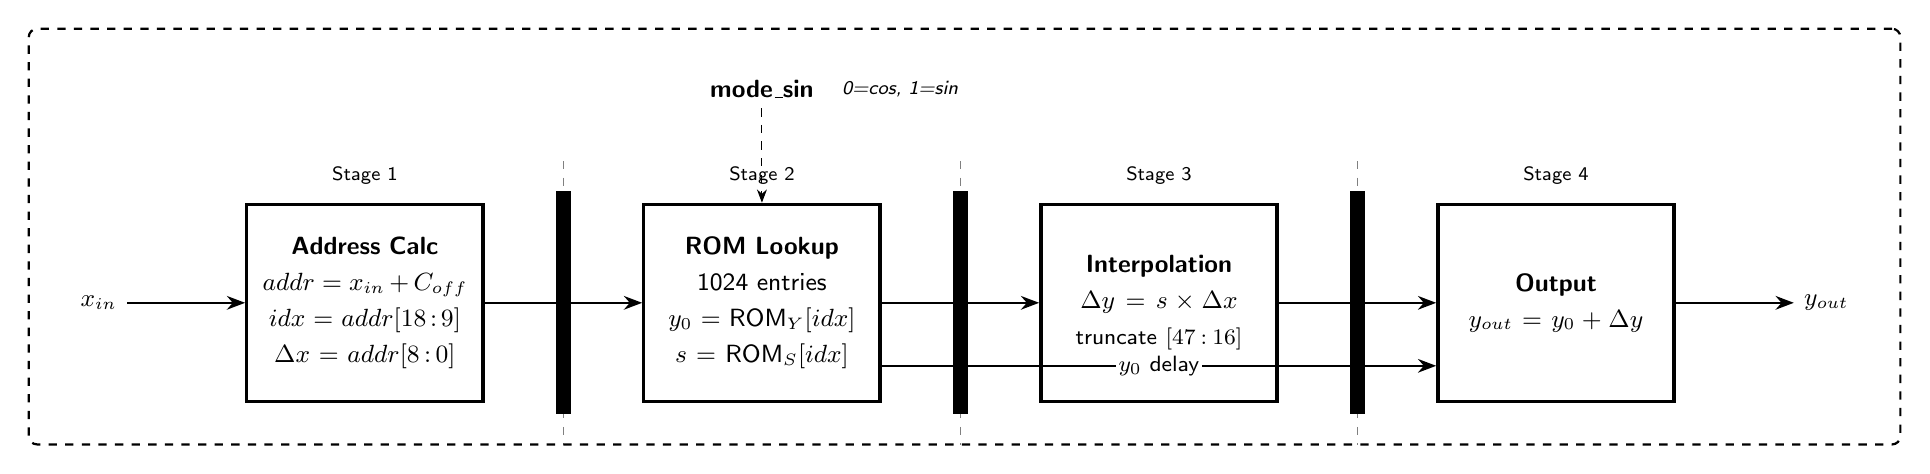
\begin{tikzpicture}[
    node distance=1.2cm and 2.0cm,
    >=Stealth, thick, font=\sffamily
]

% ---------------------------------------------------------
% Pipeline stage boxes
% ---------------------------------------------------------
\tikzset{
    pipestage/.style={
        rectangle, draw, very thick,
        minimum width=3.0cm, minimum height=2.5cm,
        font=\sffamily\small, align=center,
        text width=2.6cm
    }
}

% Stage 1: Address Calculation
\node[pipestage] (S1) at (0, 0) {%
    \textbf{Address Calc}\\[2pt]
    $addr = x_{in} + C_{off}$\\[2pt]
    $idx = addr[18\!:\!9]$\\[2pt]
    $\Delta x = addr[8\!:\!0]$
};

% Stage 2: ROM Lookup
\node[pipestage, right=2.0cm of S1] (S2) {%
    \textbf{ROM Lookup}\\[2pt]
    1024 entries\\[2pt]
    $y_0 = \text{ROM}_Y[idx]$\\[2pt]
    $s = \text{ROM}_S[idx]$
};

% Stage 3: Interpolation
\node[pipestage, right=2.0cm of S2] (S3) {%
    \textbf{Interpolation}\\[2pt]
    $\Delta y = s \times \Delta x$\\[2pt]
    {\footnotesize truncate $[47\!:\!16]$}
};

% Stage 4: Output Sum
\node[pipestage, right=2.0cm of S3] (S4) {%
    \textbf{Output}\\[2pt]
    $y_{out} = y_0 + \Delta y$
};

% ---------------------------------------------------------
% Pipeline register bars between stages
% ---------------------------------------------------------
\foreach \a/\b in {S1/S2, S2/S3, S3/S4} {
    \coordinate (mid) at ($(\a.east)!0.5!(\b.west)$);
    \draw[stage sep] ($(mid) + (0, 1.8)$) -- ($(mid) + (0, -1.8)$);
    \draw[fill=black] ($(mid) + (-0.08, 1.4)$) rectangle ($(mid) + (0.08, -1.4)$);
}

% Stage labels
\node[font=\sffamily\scriptsize, above=0.1cm of S1] {Stage 1};
\node[font=\sffamily\scriptsize, above=0.1cm of S2] {Stage 2};
\node[font=\sffamily\scriptsize, above=0.1cm of S3] {Stage 3};
\node[font=\sffamily\scriptsize, above=0.1cm of S4] {Stage 4};

% ---------------------------------------------------------
% Data flow arrows
% ---------------------------------------------------------
\draw[data arrow] (S1) -- (S2);
\draw[data arrow] (S2) -- (S3);
\draw[data arrow] (S3) -- (S4);

% Delay line for y_0 (bypass from S2 to S4)
\coordinate (bypassStart) at ($(S2.east) + (0, -0.8)$);
\coordinate (bypassEnd) at ($(S4.west) + (0, -0.8)$);
\draw[data arrow] (bypassStart) -- (bypassEnd)
    node[signal, midway] {$y_0$ delay};

% ---------------------------------------------------------
% Input / Output ports
% ---------------------------------------------------------
\node[port, left=1.5cm of S1] (xin) {$x_{in}$};
\draw[data arrow] (xin) -- (S1.west);

\node[port, right=1.5cm of S4] (yout) {$y_{out}$};
\draw[data arrow] (S4.east) -- (yout);

% Mode_sin input (top)
\node[port, above=1.2cm of S2] (mode) {mode\_sin};
\draw[ctrl arrow] (mode) -- (S2.north);
\node[const, right=0.1cm of mode] {\scriptsize 0=cos, 1=sin};

% ---------------------------------------------------------
% Dashed entity border
% ---------------------------------------------------------
\node[entity border, fit=(S1)(S4)(xin)(yout)(mode), inner sep=15pt] {};

\end{tikzpicture}%
}

\vspace{3mm}
\begin{align*}
    y_{out} &= y_0[idx] + \text{slope}[idx] \times \Delta x \quad\text{(piecewise linear interpolation)}
\end{align*}

\noindent\textit{Pipeline latency: 4 clock cycles. ROM: 1024 entries for $[-\pi, +\pi]$. Shared structure for both $\sin$ and $\cos$ via \textsf{mode\_sin} selector.}

\caption{LUT\_Trig block -- 4-stage pipelined trigonometric lookup with linear interpolation.}
\label{fig:lut_trig}
\end{figure}


\subsection{Shift Register}
\begin{figure}[H]
\centering
\resizebox{\textwidth}{!}{%
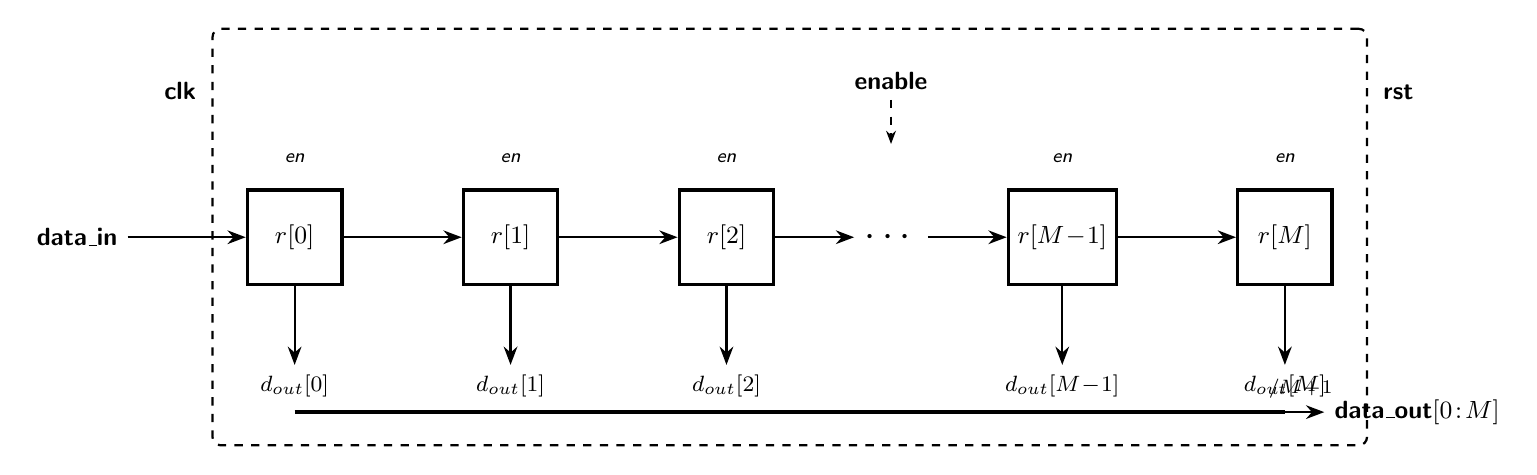
\begin{tikzpicture}[
    node distance=1.5cm and 1.8cm,
    >=Stealth, thick, font=\sffamily
]

% ---------------------------------------------------------
% Styles
% ---------------------------------------------------------
\tikzset{
    reg/.style={
        rectangle, draw, very thick,
        minimum width=1.2cm, minimum height=1.2cm,
        font=\sffamily\small, align=center
    }
}

% ---------------------------------------------------------
% Register chain
% ---------------------------------------------------------
\node[reg] (R0) at (0, 0) {$r[0]$};
\node[reg, right=1.5cm of R0] (R1) {$r[1]$};
\node[reg, right=1.5cm of R1] (R2) {$r[2]$};
\node[right=1.0cm of R2, font=\sffamily\Large] (dots) {$\cdots$};
\node[reg, right=1.0cm of dots] (RM1) {$r[M\!-\!1]$};
\node[reg, right=1.5cm of RM1] (RM) {$r[M]$};

% ---------------------------------------------------------
% Input
% ---------------------------------------------------------
\node[port, left=1.5cm of R0] (DataIn) {data\_in};
\draw[data arrow] (DataIn) -- (R0.west);

% ---------------------------------------------------------
% Arrows between registers
% ---------------------------------------------------------
\draw[data arrow] (R0) -- (R1);
\draw[data arrow] (R1) -- (R2);
\draw[data arrow] (R2) -- (dots);
\draw[data arrow] (dots) -- (RM1);
\draw[data arrow] (RM1) -- (RM);

% ---------------------------------------------------------
% Enable signal (top)
% ---------------------------------------------------------
\node[port, above=1.5cm of dots] (Enable) {enable};
\draw[ctrl arrow] (Enable) -- ++(0, -0.8);
\node[const, above=0.2cm of R0] {\scriptsize en};
\node[const, above=0.2cm of R1] {\scriptsize en};
\node[const, above=0.2cm of R2] {\scriptsize en};
\node[const, above=0.2cm of RM1] {\scriptsize en};
\node[const, above=0.2cm of RM] {\scriptsize en};

% ---------------------------------------------------------
% Output taps
% ---------------------------------------------------------
\foreach \rname/\idx in {R0/0, R1/1, R2/2, RM1/{M\!-\!1}, RM/M} {
    \draw[data arrow] (\rname.south) -- ++(0, -1.0)
        node[below, font=\sffamily\footnotesize] {$d_{out}[\idx]$};
}

% ---------------------------------------------------------
% Output bus collector
% ---------------------------------------------------------
\coordinate (busL) at ($(R0.south) + (0, -1.6)$);
\coordinate (busR) at ($(RM.south) + (0, -1.6)$);
\draw[very thick] (busL) -- (busR);
\node[port, right=0.5cm of busR] (BusOut) {data\_out$[0\!:\!M]$};
\draw[data arrow] (busR) -- (BusOut);

% Bus slash
\node[bus] at ($(busR) + (0.2, 0.3)$) {$/M\!+\!1$};

% ---------------------------------------------------------
% Clock/Reset
% ---------------------------------------------------------
\node[port, above left=1.0cm and 0.5cm of R0] (Clk) {clk};
\node[port, above right=1.0cm and 0.5cm of RM] (Rst) {rst};

% ---------------------------------------------------------
% Dashed entity border
% ---------------------------------------------------------
\node[entity border, fit=(R0)(RM)(Enable)(busL)(busR), inner sep=12pt] {};

\end{tikzpicture}%
}

\vspace{3mm}
\noindent\textit{Shift direction: new data enters at $r[0]$; oldest sample at $r[M]$. Shift occurs on rising edge of \textsf{clk} when \textsf{enable}~$= 1$.}

\caption{Shift Register block -- sliding window buffer (Generic: \textsf{DEPTH}$= M$, producing $M+1$ taps).}
\label{fig:shift_register}
\end{figure}


% ---- Stage 2 ----
\section{Stage 2: Convolutional Layer}
\begin{figure}[H]
\centering
\resizebox{\textwidth}{!}{%
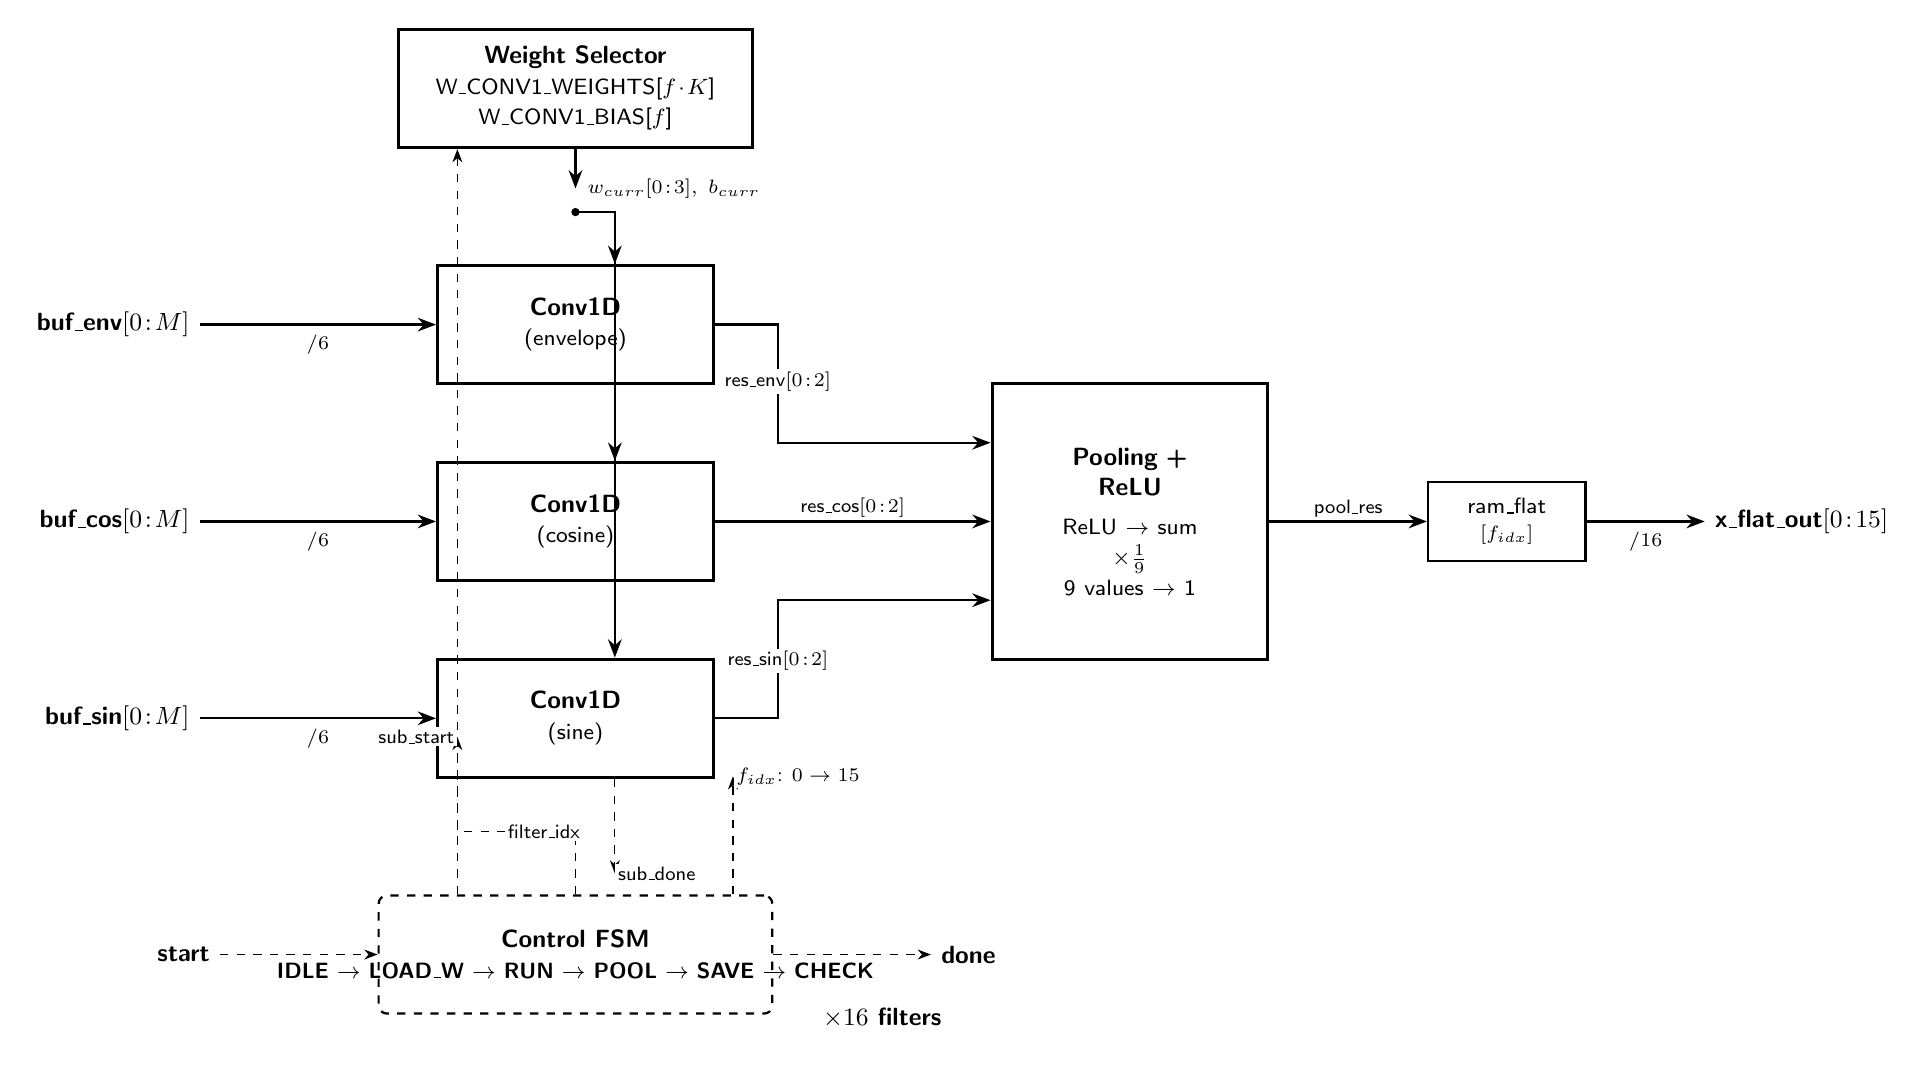
\begin{tikzpicture}[
    node distance=1.2cm and 2.0cm,
    >=Stealth, thick, font=\sffamily
]

% ---------------------------------------------------------
% Conv1D blocks (stacked vertically)
% ---------------------------------------------------------
\node[block, minimum width=3.5cm, minimum height=1.5cm, text width=3.0cm] (CE) at (0, 3.5) {%
    \textbf{Conv1D}\\
    {\footnotesize (envelope)}
};

\node[block, minimum width=3.5cm, minimum height=1.5cm, text width=3.0cm] (CC) at (0, 1.0) {%
    \textbf{Conv1D}\\
    {\footnotesize (cosine)}
};

\node[block, minimum width=3.5cm, minimum height=1.5cm, text width=3.0cm] (CS) at (0, -1.5) {%
    \textbf{Conv1D}\\
    {\footnotesize (sine)}
};

% ---------------------------------------------------------
% Input ports (left)
% ---------------------------------------------------------
\node[port, left=3.0cm of CE] (BufE) {buf\_env$[0\!:\!M]$};
\node[port, left=3.0cm of CC] (BufC) {buf\_cos$[0\!:\!M]$};
\node[port, left=3.0cm of CS] (BufS) {buf\_sin$[0\!:\!M]$};

\draw[data arrow] (BufE) -- (CE.west) node[bus, midway, below] {$/6$};
\draw[data arrow] (BufC) -- (CC.west) node[bus, midway, below] {$/6$};
\draw[data arrow] (BufS) -- (CS.west) node[bus, midway, below] {$/6$};

% ---------------------------------------------------------
% Weight ROM (top)
% ---------------------------------------------------------
\node[block, minimum width=4.5cm, minimum height=1.5cm, text width=4.0cm] (WROM) at (0, 6.5) {%
    \textbf{Weight Selector}\\
    {\footnotesize W\_CONV1\_WEIGHTS[$f \!\cdot\! K$]}\\
    {\footnotesize W\_CONV1\_BIAS[$f$]}
};

% Weight distribution
\draw[data arrow] (WROM.south) -- ++(0, -0.5)
    node[signal, right, xshift=3pt] {\scriptsize $w_{curr}[0\!:\!3],\ b_{curr}$};
\coordinate (wFork) at ($(WROM.south) + (0, -0.8)$);
\node[dot] at (wFork) {};
\draw[data arrow] (wFork) -| ($(CE.north) + (0.5, 0)$);
\draw[data arrow] (wFork) -| ($(CC.north) + (0.5, 0)$);
\draw[data arrow] (wFork) -| ($(CS.north) + (0.5, 0)$);

% ---------------------------------------------------------
% Pooling_ReLU Block (right)
% ---------------------------------------------------------
\node[block, minimum width=3.5cm, minimum height=3.5cm, text width=3.0cm, right=3.5cm of CC] (Pool) {%
    \textbf{Pooling +}\\
    \textbf{ReLU}\\[3pt]
    {\footnotesize ReLU $\rightarrow$ sum}\\
    {\footnotesize $\times \frac{1}{9}$}\\
    {\footnotesize 9 values $\rightarrow$ 1}
};

% Connections from Conv1D to Pooling
\draw[data arrow] (CE.east) -- ++(0.8, 0) |- ($(Pool.west) + (0, 1.0)$)
    node[signal, pos=0.3, above] {\scriptsize res\_env$[0\!:\!2]$};
\draw[data arrow] (CC.east) -- ($(Pool.west) + (0, 0)$)
    node[signal, midway, above] {\scriptsize res\_cos$[0\!:\!2]$};
\draw[data arrow] (CS.east) -- ++(0.8, 0) |- ($(Pool.west) + (0, -1.0)$)
    node[signal, pos=0.3, below] {\scriptsize res\_sin$[0\!:\!2]$};

% ---------------------------------------------------------
% Output RAM + output
% ---------------------------------------------------------
\node[small block, right=2.0cm of Pool] (RAM) {%
    ram\_flat\\
    {\scriptsize $[f_{idx}]$}
};
\draw[data arrow] (Pool.east) -- (RAM.west)
    node[signal, midway, above] {\scriptsize pool\_res};

\node[port, right=1.5cm of RAM] (XFlat) {x\_flat\_out$[0\!:\!15]$};
\draw[data arrow] (RAM.east) -- (XFlat) node[bus, midway, below] {$/16$};

% ---------------------------------------------------------
% Control FSM (bottom)
% ---------------------------------------------------------
\node[entity border, minimum width=5.0cm, minimum height=1.5cm] (FSM) at (0, -4.5) {};
\node[font=\sffamily\small\bfseries, align=center] at (FSM.center) {%
    Control FSM\\
    {\footnotesize IDLE $\rightarrow$ LOAD\_W $\rightarrow$ RUN $\rightarrow$ POOL $\rightarrow$ SAVE $\rightarrow$ CHECK}
};

% FSM signals
\node[port, left=2.0cm of FSM] (Start) {start};
\draw[ctrl arrow] (Start) -- (FSM.west);

\node[port, right=2.0cm of FSM] (Done) {done};
\draw[ctrl arrow] (FSM.east) -- (Done);

% Loop annotation
\draw[ctrl arrow, ->] ($(FSM.north) + (2.0, 0)$) -- ++(0, 1.5)
    node[signal, right] {\scriptsize $f_{idx}$: $0 \rightarrow 15$};

% sub_start
\draw[ctrl arrow] ($(FSM.north) + (-1.5, 0)$) -- ++(0, 2.0)
    node[signal, left] {\scriptsize sub\_start};

% sub_done feedback
\draw[ctrl arrow] ($(CS.south) + (0.5, 0)$) -- ++(0, -1.2)
    node[signal, right] {\scriptsize sub\_done};

% Filter index to weight ROM
\draw[ctrl arrow] ($(FSM.north) + (0, 0)$) -- ++(0, 0.8) -| ($(WROM.south) + (-1.5, 0)$)
    node[signal, pos=0.3, right] {\scriptsize filter\_idx};

% ---------------------------------------------------------
% Loop annotation (prominent)
% ---------------------------------------------------------
\node[annotation, font=\sffamily\small\bfseries, right=0.5cm of FSM.east, yshift=-0.8cm] {%
    $\times 16$ filters
};

% ---------------------------------------------------------
% start input
% ---------------------------------------------------------

\end{tikzpicture}%
}

\vspace{3mm}
\noindent\textit{Serialized over 16 filters: for each filter, loads shared weights, runs 3 parallel Conv1D blocks, pools the 9 results into 1 scalar. Output: 16-element feature vector \textsf{x\_flat\_out}. Generics: \textsf{N\_FILTERS}$=16$, \textsf{KERNEL\_SIZE}$=4$, \textsf{M}$=5$.}

\caption{Conv\_Layer\_Serial -- serialized 1D convolutional layer with 3 channels and 16 filters.}
\label{fig:conv_layer}
\end{figure}


\subsection{Conv1D Block}
\begin{figure}[H]
\centering
\resizebox{\textwidth}{!}{%
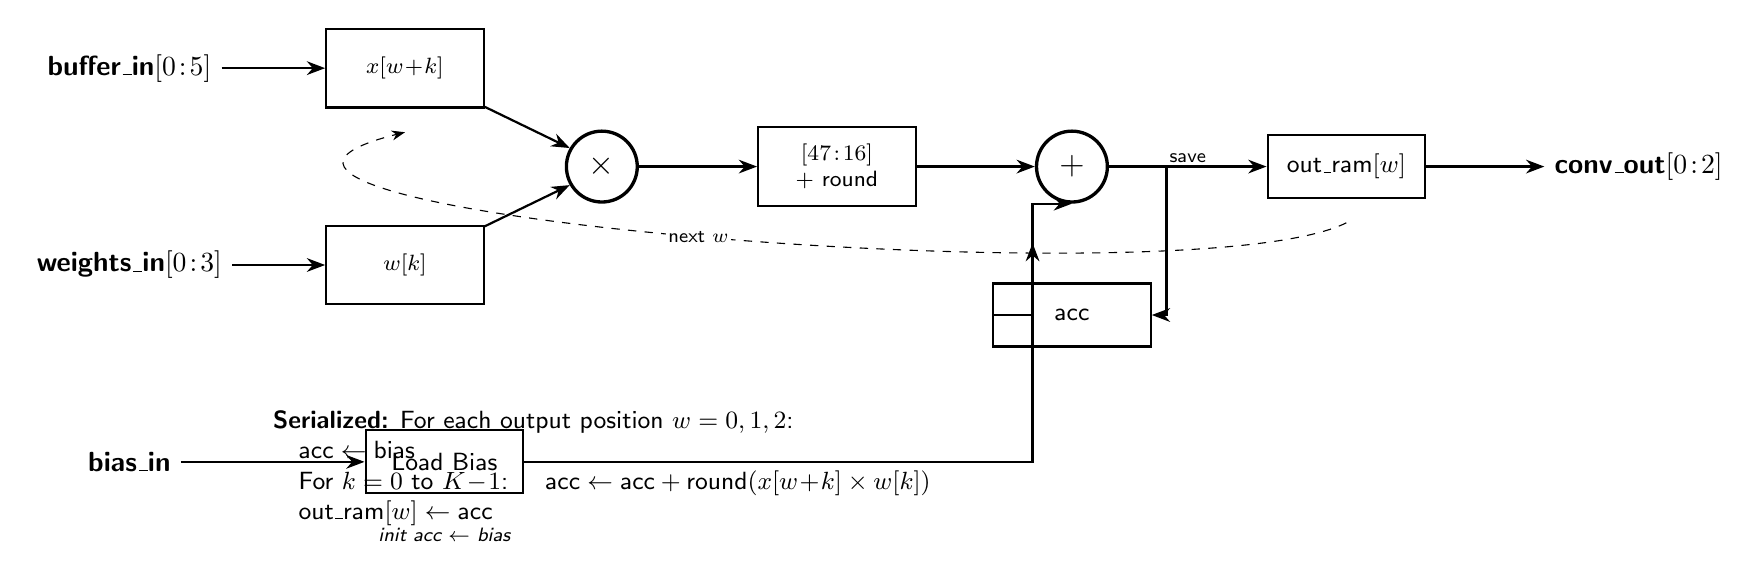
\begin{tikzpicture}[
    node distance=1.2cm and 2.0cm,
    >=Stealth, thick, font=\sffamily\large
]

% ---------------------------------------------------------
% Styles
% ---------------------------------------------------------
\tikzset{
    op_node/.style={
        circle, draw=black, very thick, minimum size=0.9cm, fill=white
    },
    io_node/.style={font=\sffamily\bfseries},
    mem/.style={
        rectangle, draw, thick,
        minimum width=2.0cm, minimum height=0.8cm,
        font=\sffamily\small, align=center
    },
    dot/.style={circle, fill=black, inner sep=0pt, minimum size=4pt}
}

% ---------------------------------------------------------
% Input ports
% ---------------------------------------------------------
\node[io_node] (BufIn) at (-6, 2.5) {buffer\_in$[0\!:\!5]$};
\node[io_node] (WIn)   at (-6, 0.0) {weights\_in$[0\!:\!3]$};
\node[io_node] (BIn)   at (-6, -2.5) {bias\_in};

% ---------------------------------------------------------
% Bias load
% ---------------------------------------------------------
\node[mem] (BiasLoad) at (-2, -2.5) {Load Bias};
\draw[data arrow] (BIn) -- (BiasLoad);

% ---------------------------------------------------------
% Multiplier: buffer[w+k] x weights[k]
% ---------------------------------------------------------
\node[op_node] (Mult) at (0, 1.25) {$\times$};

% MUX/selector for buffer[w+k]
\node[small block] (BufSel) at (-2.5, 2.5) {$x[w\!+\!k]$};
\draw[data arrow] (BufIn) -- (BufSel);
\draw[data arrow] (BufSel) -- (Mult.150);

% MUX/selector for weights[k]
\node[small block] (WSel) at (-2.5, 0.0) {$w[k]$};
\draw[data arrow] (WIn) -- (WSel);
\draw[data arrow] (WSel) -- (Mult.210);

% ---------------------------------------------------------
% Truncate + Round
% ---------------------------------------------------------
\node[small block, right=1.5cm of Mult] (Trunc) {%
    $[47\!:\!16]$\\
    + round
};
\draw[data arrow] (Mult) -- (Trunc);

% ---------------------------------------------------------
% Accumulator (adder with feedback)
% ---------------------------------------------------------
\node[op_node, right=1.5cm of Trunc] (Add) {$+$};
\draw[data arrow] (Trunc) -- (Add);

% Feedback loop
\node[mem, below=1.0cm of Add] (Acc) {acc};
\draw[data arrow] (Add) -- ++(1.2, 0) |- (Acc.east);
\draw[data arrow] (Acc.west) -| ($(Add.south) + (-0.5, 0)$) -- (Add.south);

% Bias init path
\draw[data arrow] (BiasLoad) -| ($(Add.south) + (-0.5, -0.5)$);
\node[const, below=0.3cm of BiasLoad] {\scriptsize init acc $\leftarrow$ bias};

% ---------------------------------------------------------
% Output RAM
% ---------------------------------------------------------
\node[mem, right=2.0cm of Add] (OutRAM) {out\_ram$[w]$};
\draw[data arrow] (Add) -- (OutRAM) node[signal, midway, above] {\scriptsize save};

% ---------------------------------------------------------
% Output port
% ---------------------------------------------------------
\node[io_node, right=1.5cm of OutRAM] (ConvOut) {conv\_out$[0\!:\!2]$};
\draw[data arrow] (OutRAM) -- (ConvOut);

% ---------------------------------------------------------
% Loop annotation
% ---------------------------------------------------------
\node[annotation, below=2.5cm of Mult] {%
    \textbf{Serialized:} For each output position $w = 0, 1, 2$:\\
    \quad $\text{acc} \leftarrow \text{bias}$\\
    \quad For $k = 0$ to $K\!-\!1$: \quad $\text{acc} \leftarrow \text{acc} + \text{round}(x[w\!+\!k] \times w[k])$\\
    \quad $\text{out\_ram}[w] \leftarrow \text{acc}$
};

% ---------------------------------------------------------
% FSM loop arrow
% ---------------------------------------------------------
\draw[ctrl arrow, ->] ($(OutRAM.south) + (0, -0.3)$)
    .. controls +(-2, -1.0) and +(-4, -1.0) ..
    ($(BufSel.south) + (0, -0.3)$)
    node[signal, midway] {\scriptsize next $w$};

\end{tikzpicture}%
}

\vspace{3mm}
\begin{equation*}
    \text{conv\_out}[w] = b + \sum_{k=0}^{K-1} \text{buffer}[w+k] \cdot \text{weight}[k], \quad w = 0, 1, 2
\end{equation*}

\noindent\textit{Generics: \textsf{KERNEL\_SIZE}$= 4$, \textsf{BUFFER\_SIZE}$= 6$. Output size: $6 - 4 + 1 = 3$ positions. Fixed-point truncation with round-to-nearest.}

\caption{Conv1D\_Block -- serialized 1D convolution with MAC and bias.}
\label{fig:conv1d_block}
\end{figure}


\subsection{Pooling and ReLU}
\begin{figure}[H]
\centering
\resizebox{\textwidth}{!}{%
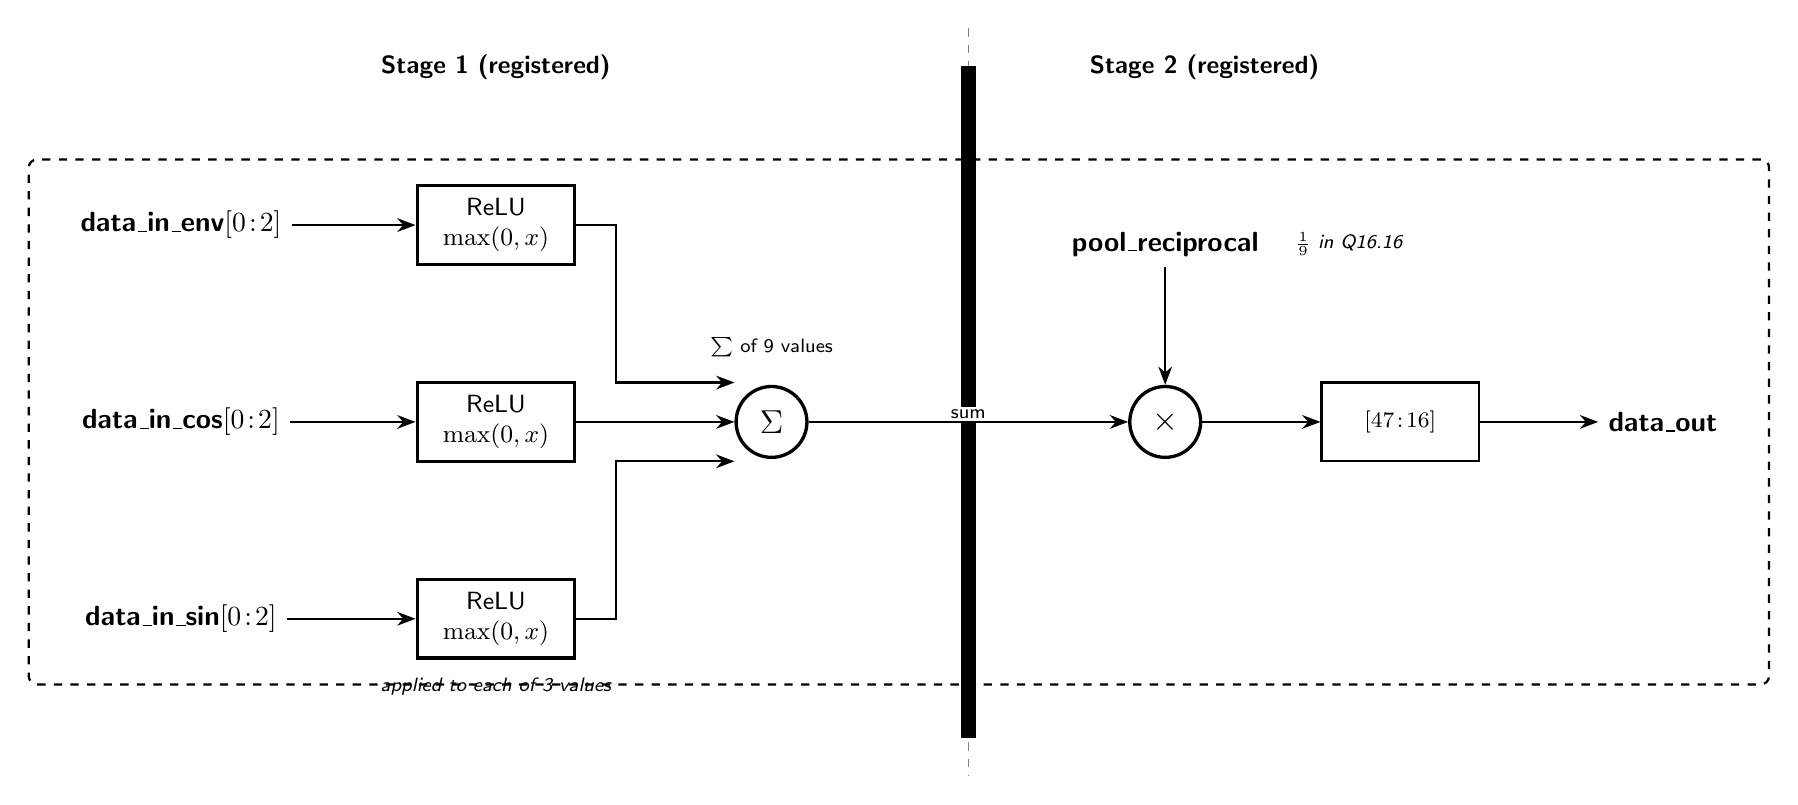
\begin{tikzpicture}[
    node distance=1.2cm and 2.5cm,
    >=Stealth, thick, font=\sffamily\large
]

% ---------------------------------------------------------
% Styles
% ---------------------------------------------------------
\tikzset{
    op_node/.style={
        circle, draw=black, very thick, minimum size=0.9cm, fill=white
    },
    io_node/.style={font=\sffamily\bfseries},
    relu_box/.style={
        rectangle, draw, very thick,
        minimum width=2.0cm, minimum height=1.0cm,
        font=\sffamily\small, align=center
    },
    dot/.style={circle, fill=black, inner sep=0pt, minimum size=4pt}
}

% ---------------------------------------------------------
% Stage labels
% ---------------------------------------------------------
\node[font=\sffamily\small\bfseries] at (-3.5, 4.5) {Stage 1 (registered)};
\node[font=\sffamily\small\bfseries] at (5.5, 4.5) {Stage 2 (registered)};

% Stage separator
\draw[stage sep] (2.5, 5.0) -- (2.5, -4.5);
\draw[fill=black] (2.42, 4.5) rectangle (2.58, -4.0);

% ---------------------------------------------------------
% Inputs (left side)
% ---------------------------------------------------------
\node[io_node] (InEnv) at (-7.5, 2.5) {data\_in\_env$[0\!:\!2]$};
\node[io_node] (InCos) at (-7.5, 0.0) {data\_in\_cos$[0\!:\!2]$};
\node[io_node] (InSin) at (-7.5, -2.5) {data\_in\_sin$[0\!:\!2]$};

% ---------------------------------------------------------
% ReLU blocks (one per channel)
% ---------------------------------------------------------
\node[relu_box] (ReLU_E) at (-3.5, 2.5) {ReLU\\$\max(0, x)$};
\node[relu_box] (ReLU_C) at (-3.5, 0.0) {ReLU\\$\max(0, x)$};
\node[relu_box] (ReLU_S) at (-3.5, -2.5) {ReLU\\$\max(0, x)$};

\draw[data arrow] (InEnv) -- (ReLU_E);
\draw[data arrow] (InCos) -- (ReLU_C);
\draw[data arrow] (InSin) -- (ReLU_S);

% Annotation: applied to all 3 values per channel
\node[const, below=0.1cm of ReLU_S] {\scriptsize applied to each of 3 values};

% ---------------------------------------------------------
% Summation (all 9 values)
% ---------------------------------------------------------
\node[op_node] (Sum) at (0.0, 0.0) {$\Sigma$};

\draw[data arrow] (ReLU_E.east) -- ++(0.5, 0) |- ($(Sum.west) + (0, 0.5)$);
\draw[data arrow] (ReLU_C.east) -- (Sum.west);
\draw[data arrow] (ReLU_S.east) -- ++(0.5, 0) |- ($(Sum.west) + (0, -0.5)$);

\node[signal, above=0.3cm of Sum] {\scriptsize $\sum$ of 9 values};

% ---------------------------------------------------------
% Stage 2: Multiply by reciprocal
% ---------------------------------------------------------
\node[op_node] (Mult) at (5.0, 0.0) {$\times$};

\draw[data arrow] (Sum) -- (Mult) node[signal, midway, above] {\scriptsize sum};

% Reciprocal input from top
\node[io_node, above=1.5cm of Mult] (Recip) {pool\_reciprocal};
\draw[data arrow] (Recip) -- (Mult);
\node[const, right=0.2cm of Recip] {\scriptsize $\frac{1}{9}$ in Q16.16};

% ---------------------------------------------------------
% Truncate
% ---------------------------------------------------------
\node[small block, right=1.5cm of Mult] (Trunc) {$[47\!:\!16]$};
\draw[data arrow] (Mult) -- (Trunc);

% ---------------------------------------------------------
% Output
% ---------------------------------------------------------
\node[io_node, right=1.5cm of Trunc] (Out) {data\_out};
\draw[data arrow] (Trunc) -- (Out);

% ---------------------------------------------------------
% Entity border
% ---------------------------------------------------------
\node[entity border, fit=(InEnv)(InSin)(Out)(Recip), inner sep=15pt] {};

\end{tikzpicture}%
}

\vspace{3mm}
\begin{equation*}
    \text{data\_out} = \frac{1}{3 \times W_{out}} \sum_{c \in \{\text{env}, \text{cos}, \text{sin}\}} \sum_{i=0}^{W_{out}-1} \text{ReLU}(x_{c,i})
\end{equation*}

\noindent\textit{Generic: \textsf{INPUT\_SIZE}$= 3$ ($W_{out}$). Total 9 values pooled into 1 scalar. 2-stage registered pipeline.}

\caption{Pooling\_ReLU\_Block -- ReLU activation followed by global average pooling across 3 channels.}
\label{fig:pooling_relu}
\end{figure}


% ---- Stage 3 ----
\section{Stage 3: MLP Backend}
\begin{figure}[H]
\centering
\resizebox{\textwidth}{!}{%
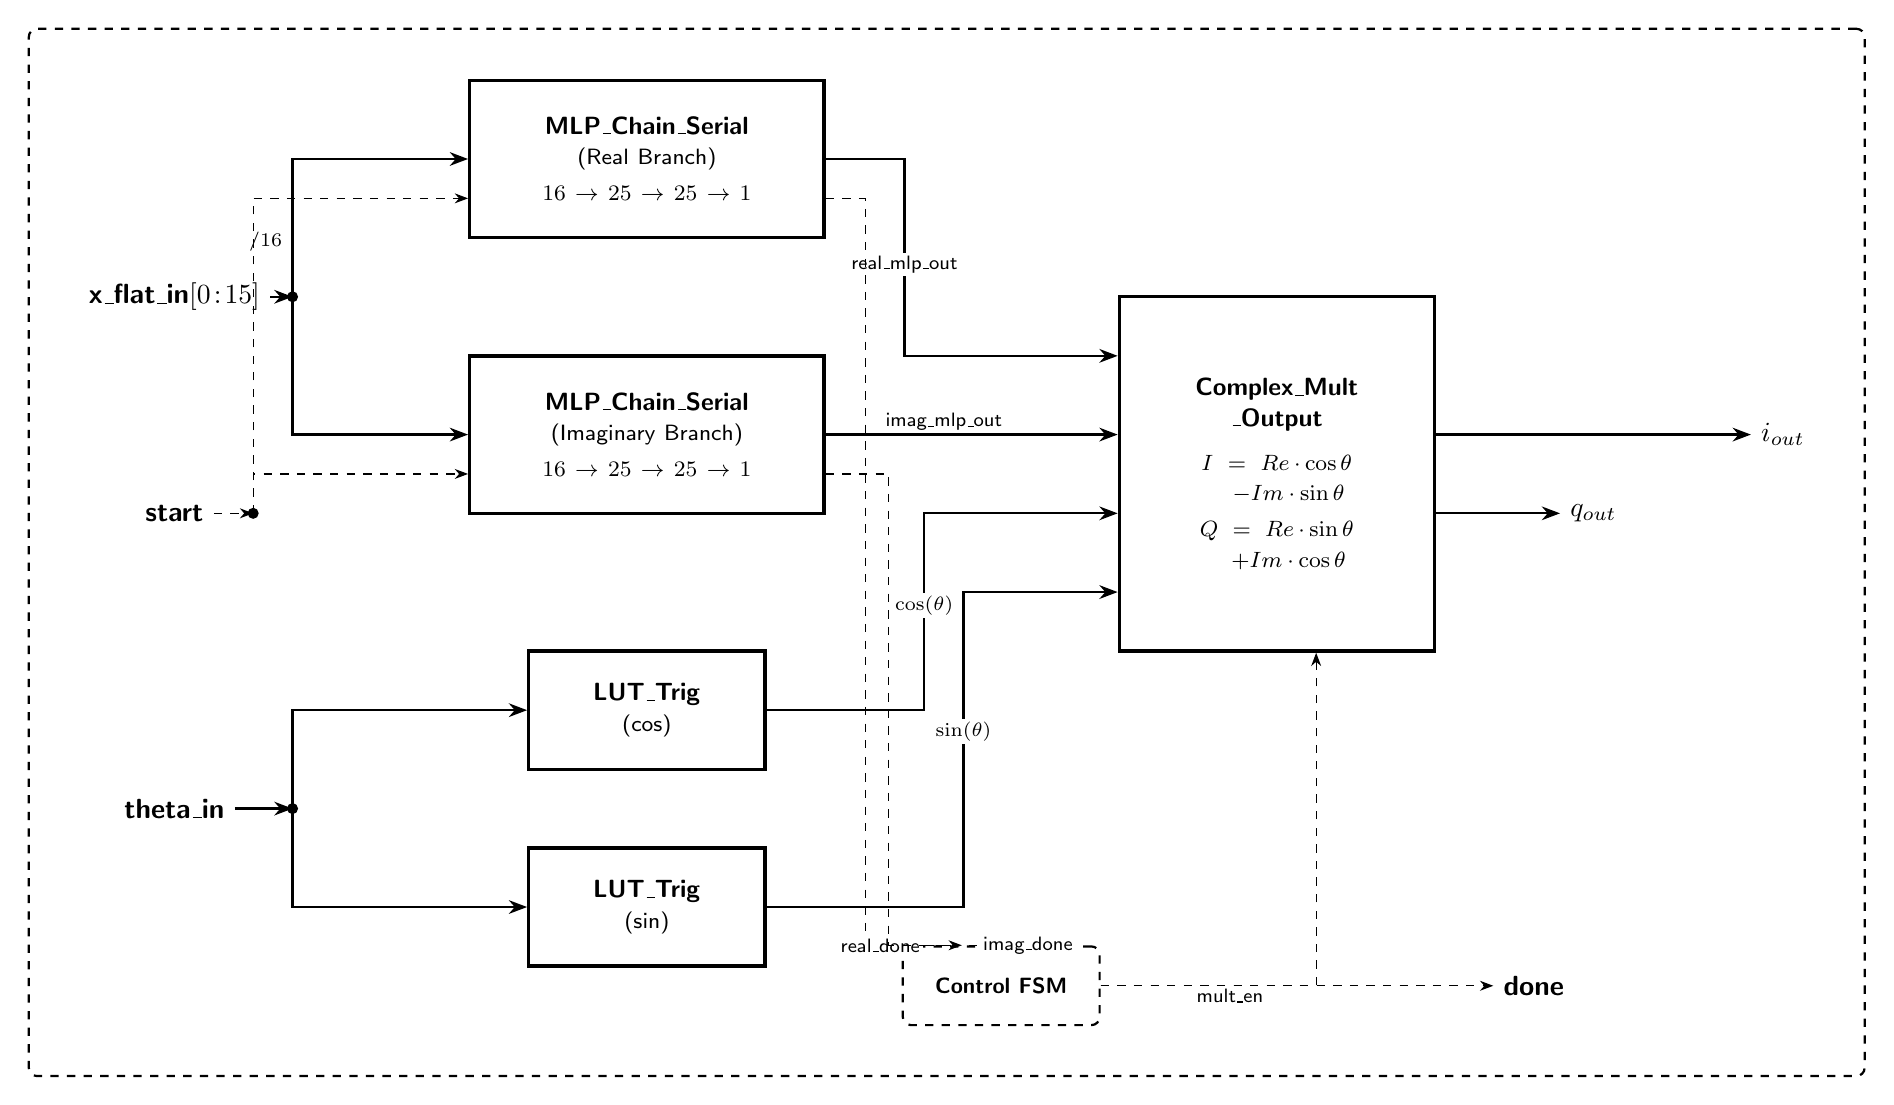
\begin{tikzpicture}[
    node distance=1.5cm and 2.0cm,
    >=Stealth, thick, font=\sffamily
]

% ---------------------------------------------------------
% Styles
% ---------------------------------------------------------
\tikzset{
    io_node/.style={font=\sffamily\bfseries},
    dot/.style={circle, fill=black, inner sep=0pt, minimum size=4pt}
}

% ---------------------------------------------------------
% MLP blocks (stacked vertically, left side)
% ---------------------------------------------------------
\node[block, minimum width=4.5cm, minimum height=2.0cm, text width=4.0cm] (MLP_R) at (0, 3.0) {%
    \textbf{MLP\_Chain\_Serial}\\
    {\footnotesize (Real Branch)}\\[2pt]
    {\footnotesize $16 \!\rightarrow\! 25 \!\rightarrow\! 25 \!\rightarrow\! 1$}
};

\node[block, minimum width=4.5cm, minimum height=2.0cm, text width=4.0cm] (MLP_I) at (0, -0.5) {%
    \textbf{MLP\_Chain\_Serial}\\
    {\footnotesize (Imaginary Branch)}\\[2pt]
    {\footnotesize $16 \!\rightarrow\! 25 \!\rightarrow\! 25 \!\rightarrow\! 1$}
};

% ---------------------------------------------------------
% LUT Trig blocks (below MLPs)
% ---------------------------------------------------------
\node[block, minimum width=3.0cm, minimum height=1.5cm, text width=2.5cm] (LUT_C) at (0, -4.0) {%
    \textbf{LUT\_Trig}\\
    {\footnotesize (cos)}
};

\node[block, minimum width=3.0cm, minimum height=1.5cm, text width=2.5cm] (LUT_S) at (0, -6.5) {%
    \textbf{LUT\_Trig}\\
    {\footnotesize (sin)}
};

% ---------------------------------------------------------
% Complex_Mult_Output (right side)
% ---------------------------------------------------------
\node[block, minimum width=4.0cm, minimum height=4.5cm, text width=3.5cm] (CMult) at (8.0, -1.0) {%
    \textbf{Complex\_Mult}\\
    \textbf{\_Output}\\[5pt]
    {\footnotesize $I = Re \!\cdot\! \cos\theta$}\\
    {\footnotesize $\quad - Im \!\cdot\! \sin\theta$}\\[2pt]
    {\footnotesize $Q = Re \!\cdot\! \sin\theta$}\\
    {\footnotesize $\quad + Im \!\cdot\! \cos\theta$}
};

% ---------------------------------------------------------
% Input: x_flat_in (far left, feeds both MLPs)
% ---------------------------------------------------------
\node[io_node] (XFlat) at (-6.0, 1.25) {x\_flat\_in$[0\!:\!15]$};
\draw[data arrow] (XFlat) -- ++(1.5, 0) coordinate (xFork);
\node[dot] at (xFork) {};
\draw[data arrow] (xFork) |- (MLP_R.west)
    node[bus, pos=0.2, left] {$/16$};
\draw[data arrow] (xFork) |- (MLP_I.west);

% ---------------------------------------------------------
% Input: theta_in (far left, feeds both LUTs)
% ---------------------------------------------------------
\node[io_node] (Theta) at (-6.0, -5.25) {theta\_in};
\draw[data arrow] (Theta) -- ++(1.5, 0) coordinate (tFork);
\node[dot] at (tFork) {};
\draw[data arrow] (tFork) |- (LUT_C.west);
\draw[data arrow] (tFork) |- (LUT_S.west);

% ---------------------------------------------------------
% Input: start
% ---------------------------------------------------------
\node[io_node] (Start) at (-6.0, -1.5) {start};
\draw[ctrl arrow] (Start) -- ++(1.0, 0) coordinate (sFork);
\node[dot] at (sFork) {};
\draw[ctrl arrow] (sFork) |- ($(MLP_R.west) + (0, -0.5)$);
\draw[ctrl arrow] (sFork) |- ($(MLP_I.west) + (0, -0.5)$);

% ---------------------------------------------------------
% MLP outputs -> Complex_Mult
% ---------------------------------------------------------
\draw[data arrow] (MLP_R.east) -- ++(1.0, 0) |- ($(CMult.west) + (0, 1.5)$)
    node[signal, pos=0.3, above] {\scriptsize real\_mlp\_out};

\draw[data arrow] (MLP_I.east) -- ++(1.5, 0) |- ($(CMult.west) + (0, 0.5)$)
    node[signal, pos=0.3, above] {\scriptsize imag\_mlp\_out};

% ---------------------------------------------------------
% LUT outputs -> Complex_Mult
% ---------------------------------------------------------
\draw[data arrow] (LUT_C.east) -- ++(2.0, 0) |- ($(CMult.west) + (0, -0.5)$)
    node[signal, pos=0.3, below] {\scriptsize $\cos(\theta)$};

\draw[data arrow] (LUT_S.east) -- ++(2.5, 0) |- ($(CMult.west) + (0, -1.5)$)
    node[signal, pos=0.3, below] {\scriptsize $\sin(\theta)$};

% ---------------------------------------------------------
% Control: done signals
% ---------------------------------------------------------
% MLP done -> FSM -> mult_en
\node[entity border, minimum width=2.5cm, minimum height=1.0cm] (FSM) at (4.5, -7.5) {};
\node[font=\sffamily\footnotesize\bfseries] at (FSM.center) {Control FSM};

\draw[ctrl arrow] ($(MLP_R.east) + (0, -0.5)$) -- ++(0.5, 0) |- ($(FSM.north) + (-0.5, 0)$)
    node[signal, pos=0.8, left] {\scriptsize real\_done};
\draw[ctrl arrow] ($(MLP_I.east) + (0, -0.5)$) -- ++(0.8, 0) |- ($(FSM.north) + (0.5, 0)$)
    node[signal, pos=0.8, right] {\scriptsize imag\_done};

\draw[ctrl arrow] (FSM.east) -| ($(CMult.south) + (0.5, 0)$)
    node[signal, pos=0.3, below] {\scriptsize mult\_en};

% ---------------------------------------------------------
% Outputs (far right)
% ---------------------------------------------------------
\node[io_node, right=2.0cm of CMult] (Iout) at ($(CMult.east) + (2.0, 0.5)$) {$i_{out}$};
\node[io_node] (Qout) at ($(CMult.east) + (2.0, -0.5)$) {$q_{out}$};

\draw[data arrow] ($(CMult.east) + (0, 0.5)$) -- (Iout);
\draw[data arrow] ($(CMult.east) + (0, -0.5)$) -- (Qout);

\node[io_node] (DoneOut) at ($(FSM.east) + (5.5, 0)$) {done};
\draw[ctrl arrow] (FSM.east) -- ++(0.5, 0) |- (DoneOut);

% ---------------------------------------------------------
% Entity border
% ---------------------------------------------------------
\node[entity border, fit=(XFlat)(Theta)(Start)(Iout)(Qout)(DoneOut)(LUT_S)(FSM)(MLP_R), inner sep=18pt] {};

\end{tikzpicture}%
}

\vspace{3mm}
\begin{align*}
    i_{out} &= \text{Re}_{\text{MLP}} \cdot \cos(\theta) - \text{Im}_{\text{MLP}} \cdot \sin(\theta) \\
    q_{out} &= \text{Re}_{\text{MLP}} \cdot \sin(\theta) + \text{Im}_{\text{MLP}} \cdot \cos(\theta)
\end{align*}

\noindent\textit{Both MLP branches run in parallel. LUT\_Trig computes $\cos/\sin$ of the captured phase. Complex multiplication rotates the MLP output to reconstruct the pre-distorted IQ signal.}

\caption{BackEnd\_Wrapper -- dual MLP branches with phase rotation output stage.}
\label{fig:backend_wrapper}
\end{figure}


\subsection{MLP Chain}
\begin{figure}[H]
\centering
\resizebox{\textwidth}{!}{%
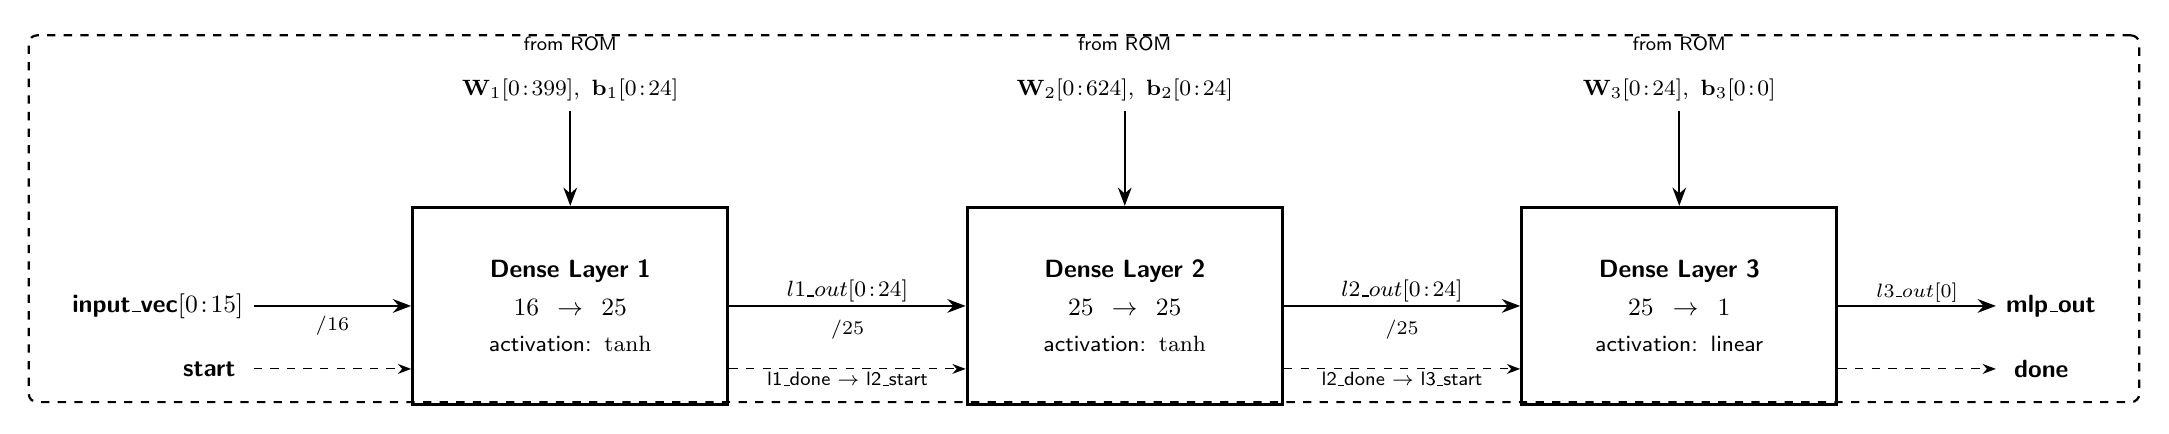
\begin{tikzpicture}[
    node distance=1.5cm and 2.5cm,
    >=Stealth, thick, font=\sffamily
]

% ---------------------------------------------------------
% Dense Layer blocks (chain)
% ---------------------------------------------------------
\node[block, minimum width=4.0cm, minimum height=2.5cm, text width=3.5cm] (L1) at (0, 0) {%
    \textbf{Dense Layer 1}\\[3pt]
    $16 \rightarrow 25$\\[2pt]
    {\footnotesize activation: $\tanh$}
};

\node[block, minimum width=4.0cm, minimum height=2.5cm, text width=3.5cm, right=3.0cm of L1] (L2) {%
    \textbf{Dense Layer 2}\\[3pt]
    $25 \rightarrow 25$\\[2pt]
    {\footnotesize activation: $\tanh$}
};

\node[block, minimum width=4.0cm, minimum height=2.5cm, text width=3.5cm, right=3.0cm of L2] (L3) {%
    \textbf{Dense Layer 3}\\[3pt]
    $25 \rightarrow 1$\\[2pt]
    {\footnotesize activation: linear}
};

% ---------------------------------------------------------
% Data flow between layers
% ---------------------------------------------------------
\draw[data arrow] (L1.east) -- (L2.west)
    node[signal, midway, above] {$l1\_out[0\!:\!24]$};
\draw[data arrow] (L2.east) -- (L3.west)
    node[signal, midway, above] {$l2\_out[0\!:\!24]$};

% Bus width marks
\node[bus] at ($(L1.east)!0.5!(L2.west) + (0, -0.3)$) {$/25$};
\node[bus] at ($(L2.east)!0.5!(L3.west) + (0, -0.3)$) {$/25$};

% ---------------------------------------------------------
% Handshake signals (start/done chain)
% ---------------------------------------------------------
% start -> L1
\coordinate (startWire) at ($(L1.west) + (-2.0, -0.8)$);
\node[port, left=0.1cm of startWire] {start};
\draw[ctrl arrow] (startWire) -- ($(L1.west) + (0, -0.8)$);

% L1.done -> L2.start
\draw[ctrl arrow] ($(L1.east) + (0, -0.8)$) -- ($(L2.west) + (0, -0.8)$)
    node[signal, midway, below] {\scriptsize l1\_done $\rightarrow$ l2\_start};

% L2.done -> L3.start
\draw[ctrl arrow] ($(L2.east) + (0, -0.8)$) -- ($(L3.west) + (0, -0.8)$)
    node[signal, midway, below] {\scriptsize l2\_done $\rightarrow$ l3\_start};

% L3.done -> done output
\coordinate (doneWire) at ($(L3.east) + (2.0, -0.8)$);
\node[port, right=0.1cm of doneWire] {done};
\draw[ctrl arrow] ($(L3.east) + (0, -0.8)$) -- (doneWire);

% ---------------------------------------------------------
% Input port (left)
% ---------------------------------------------------------
\node[port, left=2.0cm of L1] (VecIn) {input\_vec$[0\!:\!15]$};
\draw[data arrow] (VecIn) -- (L1.west)
    node[bus, midway, below] {$/16$};

% ---------------------------------------------------------
% Output port (right)
% ---------------------------------------------------------
\node[port, right=2.0cm of L3] (MlpOut) {mlp\_out};
\draw[data arrow] (L3.east) -- (MlpOut)
    node[signal, midway, above] {\scriptsize $l3\_out[0]$};

% ---------------------------------------------------------
% Weight/bias inputs (from top, per layer)
% ---------------------------------------------------------
\node[const, above=1.2cm of L1] (W1) {$\mathbf{W}_1[0\!:\!399],\ \mathbf{b}_1[0\!:\!24]$};
\draw[data arrow] (W1) -- (L1.north);
\node[font=\sffamily\scriptsize, above=0.1cm of W1] {from ROM};

\node[const, above=1.2cm of L2] (W2) {$\mathbf{W}_2[0\!:\!624],\ \mathbf{b}_2[0\!:\!24]$};
\draw[data arrow] (W2) -- (L2.north);
\node[font=\sffamily\scriptsize, above=0.1cm of W2] {from ROM};

\node[const, above=1.2cm of L3] (W3) {$\mathbf{W}_3[0\!:\!24],\ \mathbf{b}_3[0\!:\!0]$};
\draw[data arrow] (W3) -- (L3.north);
\node[font=\sffamily\scriptsize, above=0.1cm of W3] {from ROM};

% ---------------------------------------------------------
% Entity border
% ---------------------------------------------------------
\node[entity border, fit=(VecIn)(MlpOut)(W1)(W2)(W3)(startWire)(doneWire), inner sep=12pt] {};

\end{tikzpicture}%
}

\vspace{3mm}
\noindent\textit{Sequential execution: Layer 1 completes $\rightarrow$ triggers Layer 2 $\rightarrow$ triggers Layer 3. Start/done handshake between layers. Weights and biases loaded from \textsf{pkg\_model\_constants}.}

\caption{MLP\_Chain\_Serial -- 3-layer fully-connected network ($16 \!\rightarrow\! 25 \!\rightarrow\! 25 \!\rightarrow\! 1$).}
\label{fig:mlp_chain}
\end{figure}


\subsection{Dense Layer}
\begin{figure}[H]
\centering
\resizebox{\textwidth}{!}{%
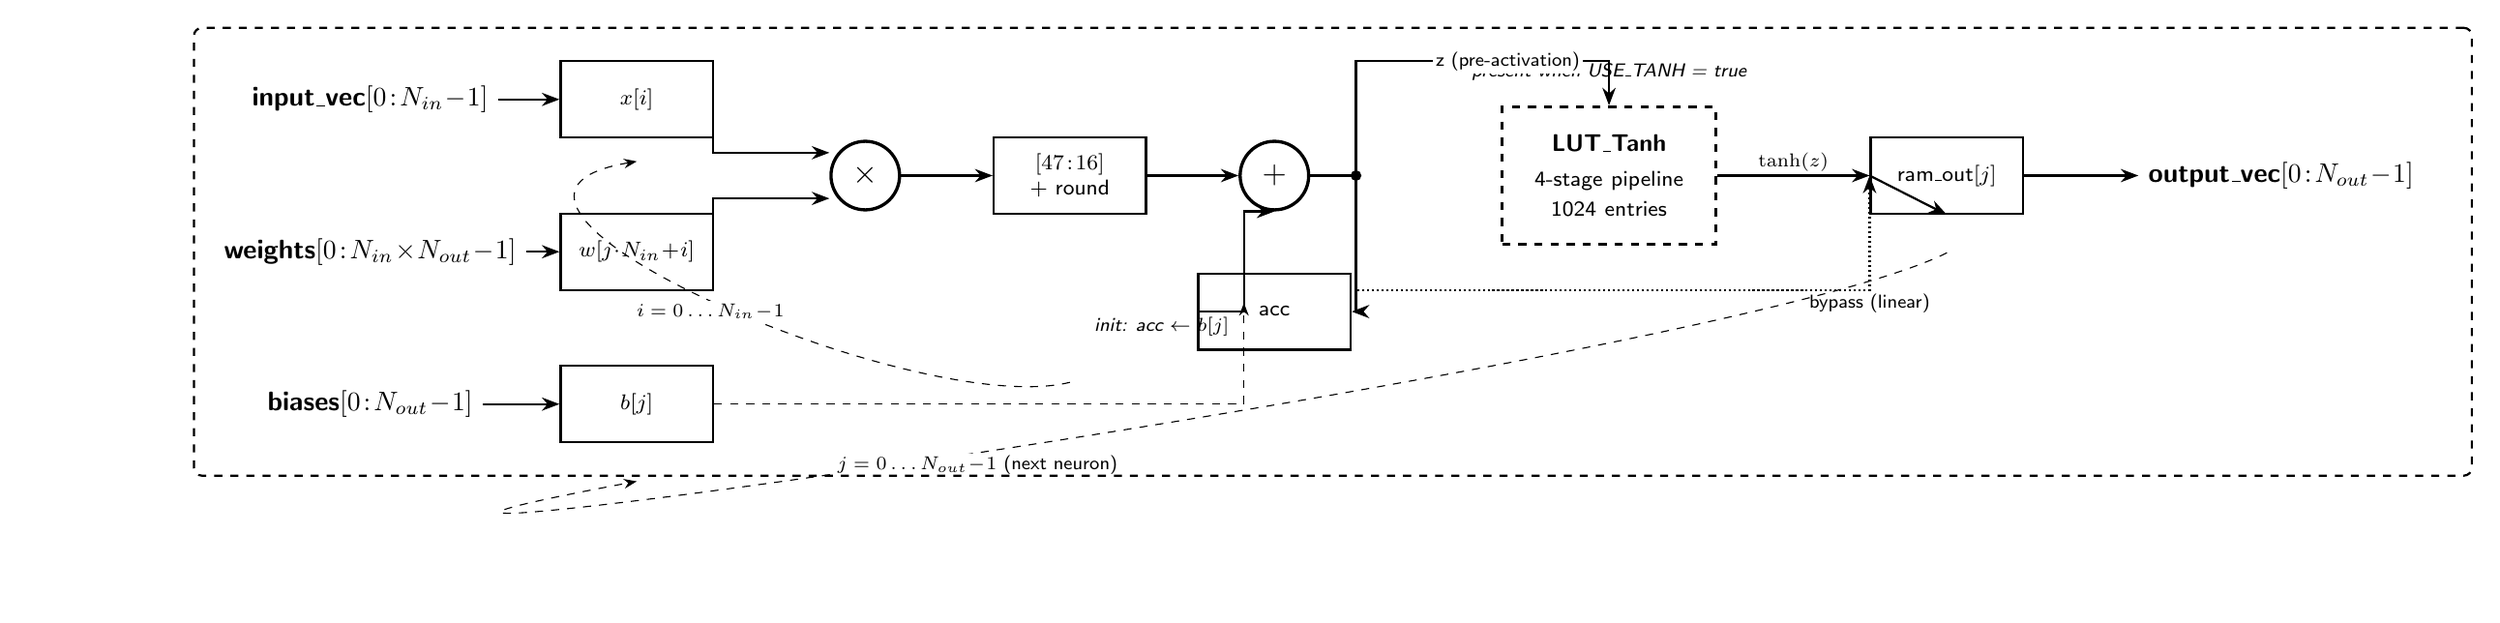
\begin{tikzpicture}[
    node distance=1.2cm and 2.0cm,
    >=Stealth, thick, font=\sffamily
]

% ---------------------------------------------------------
% Styles
% ---------------------------------------------------------
\tikzset{
    op_node/.style={
        circle, draw=black, very thick, minimum size=0.9cm, fill=white,
        font=\sffamily\large
    },
    io_node/.style={font=\sffamily\bfseries},
    dot/.style={circle, fill=black, inner sep=0pt, minimum size=4pt}
}

% ---------------------------------------------------------
% Input ports (left)
% ---------------------------------------------------------
\node[io_node] (VecIn) at (-7, 2.0) {input\_vec$[0\!:\!N_{in}\!-\!1]$};
\node[io_node] (WIn)   at (-7, 0.0) {weights$[0\!:\!N_{in} \!\times\! N_{out}\!-\!1]$};
\node[io_node] (BIn)   at (-7, -2.0) {biases$[0\!:\!N_{out}\!-\!1]$};

% ---------------------------------------------------------
% Index selectors
% ---------------------------------------------------------
\node[small block] (XSel) at (-3.5, 2.0) {$x[i]$};
\node[small block] (WSel) at (-3.5, 0.0) {$w[j \!\cdot\! N_{in} \!+\! i]$};
\node[small block] (BSel) at (-3.5, -2.0) {$b[j]$};

\draw[data arrow] (VecIn) -- (XSel);
\draw[data arrow] (WIn)   -- (WSel);
\draw[data arrow] (BIn)   -- (BSel);

% ---------------------------------------------------------
% Multiplier
% ---------------------------------------------------------
\node[op_node] (Mult) at (-0.5, 1.0) {$\times$};
\draw[data arrow] (XSel) -- ++(1.0, 0) |- ($(Mult.west) + (0, 0.3)$);
\draw[data arrow] (WSel) -- ++(1.0, 0) |- ($(Mult.west) + (0, -0.3)$);

% ---------------------------------------------------------
% Truncate + Round
% ---------------------------------------------------------
\node[small block, right=1.2cm of Mult] (Trunc) {%
    $[47\!:\!16]$\\
    + round
};
\draw[data arrow] (Mult) -- (Trunc);

% ---------------------------------------------------------
% Accumulator
% ---------------------------------------------------------
\node[op_node, right=1.2cm of Trunc] (Add) {$+$};
\draw[data arrow] (Trunc) -- (Add);

% Feedback
\node[small block, below=0.8cm of Add] (Acc) {acc};
\draw[data arrow] (Add.east) -- ++(0.6, 0) |- (Acc.east);
\draw[data arrow] (Acc.west) -| ($(Add.south) + (-0.4, 0)$) -- (Add.south);

% Bias init
\draw[ctrl arrow] (BSel) -| ($(Add.south) + (-0.4, -1.2)$)
    node[const, below left=0.1cm] {\scriptsize init: acc $\leftarrow$ $b[j]$};

% MAC loop annotation
\draw[ctrl arrow, ->] ($(Trunc.south) + (0, -2.2)$)
    .. controls +(-2, -0.5) and +(-3, -0.5) ..
    ($(XSel.south) + (0, -0.3)$)
    node[signal, midway, below] {\scriptsize $i = 0 \ldots N_{in}\!-\!1$};

% ---------------------------------------------------------
% Activation: LUT_Tanh (conditional)
% ---------------------------------------------------------
\node[block, dashed, minimum width=2.8cm, minimum height=1.8cm, text width=2.4cm,
    right=2.5cm of Add] (LUT) {%
    \textbf{LUT\_Tanh}\\[2pt]
    {\footnotesize 4-stage pipeline}\\
    {\footnotesize 1024 entries}
};
% Dashed annotation
\node[const, above=0.2cm of LUT] {\scriptsize present when USE\_TANH = true};

\draw[data arrow] (Add.east) -- ++(0.6, 0) -- ++(0, 1.5) -| (LUT.north)
    node[signal, pos=0.3] {\scriptsize z (pre-activation)};

% Bypass (linear mode)
\coordinate (BypassStart) at ($(Add.east) + (0.6, 0)$);
\node[dot] at (BypassStart) {};
\coordinate (BypassEnd) at ($(LUT.east) + (2.0, 0)$);
\draw[data arrow, densely dotted] (BypassStart) -- ++(0, -1.5) -| (BypassEnd)
    node[signal, pos=0.5, below] {\scriptsize bypass (linear)};

% ---------------------------------------------------------
% Output RAM
% ---------------------------------------------------------
\node[small block, right=2.0cm of LUT] (OutRAM) {ram\_out$[j]$};
\draw[data arrow] (LUT) -- (OutRAM) node[signal, midway, above] {\scriptsize $\tanh(z)$};
\draw[data arrow] (BypassEnd) -- (OutRAM.south);

% ---------------------------------------------------------
% Output port
% ---------------------------------------------------------
\node[io_node, right=1.5cm of OutRAM] (VecOut) {output\_vec$[0\!:\!N_{out}\!-\!1]$};
\draw[data arrow] (OutRAM) -- (VecOut);

% ---------------------------------------------------------
% Neuron loop annotation
% ---------------------------------------------------------
\draw[ctrl arrow, ->] ($(OutRAM.south) + (0, -0.5)$)
    .. controls +(-3, -1.5) and +(-8, -1.5) ..
    ($(BSel.south) + (0, -0.5)$)
    node[signal, midway, below] {\scriptsize $j = 0 \ldots N_{out}\!-\!1$ (next neuron)};

% ---------------------------------------------------------
% Entity border
% ---------------------------------------------------------
\node[entity border, fit=(VecIn)(BIn)(VecOut)(LUT), inner sep=18pt] {};

\end{tikzpicture}%
}

\vspace{3mm}
\begin{equation*}
    \text{out}[j] = f\!\left(b_j + \sum_{i=0}^{N_{in}-1} w_{j,i} \cdot x_i \right), \quad
    f = \begin{cases} \tanh & \text{if USE\_TANH} = \texttt{true} \\ \text{identity} & \text{otherwise} \end{cases}
\end{equation*}

\noindent\textit{Serialized: one neuron at a time. MAC loop with round-to-nearest. Shared single LUT\_Tanh instance (4-cycle latency). Generics: \textsf{NUM\_INPUTS}, \textsf{NUM\_OUTPUTS}, \textsf{USE\_TANH}.}

\caption{Dense\_Layer block -- fully-connected layer with serialized MAC and optional $\tanh$ activation.}
\label{fig:dense_layer}
\end{figure}


\subsection{Tanh LUT}
\begin{figure}[H]
\centering
\resizebox{\textwidth}{!}{%
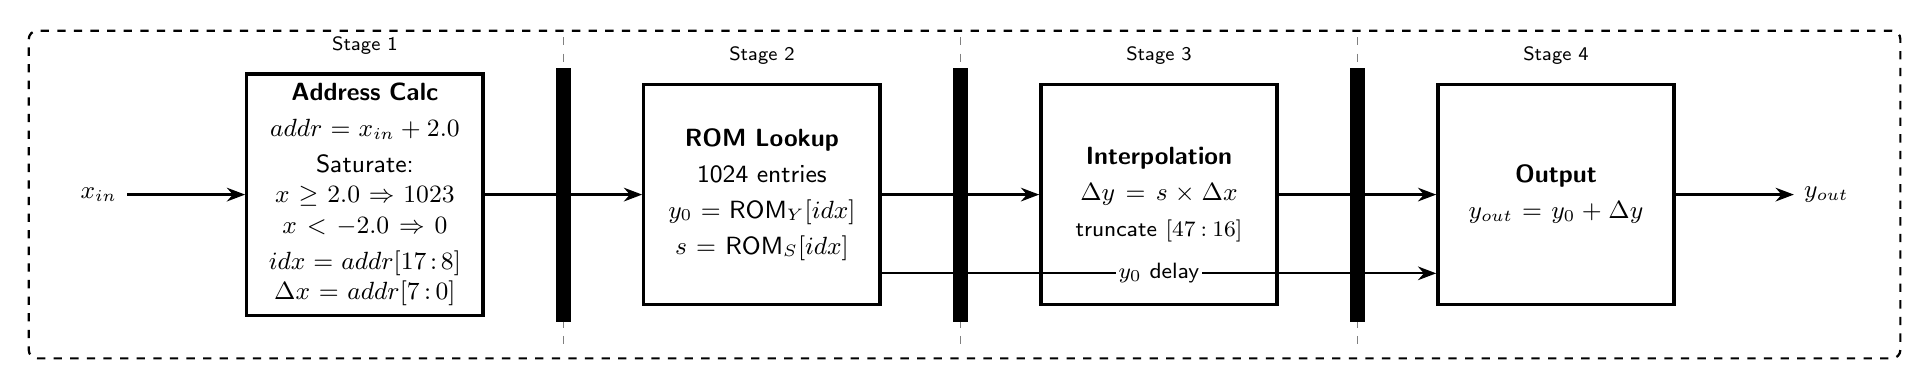
\begin{tikzpicture}[
    node distance=1.2cm and 2.0cm,
    >=Stealth, thick, font=\sffamily
]

% ---------------------------------------------------------
% Pipeline stage boxes
% ---------------------------------------------------------
\tikzset{
    pipestage/.style={
        rectangle, draw, very thick,
        minimum width=3.0cm, minimum height=2.8cm,
        font=\sffamily\small, align=center,
        text width=2.6cm
    }
}

% Stage 1: Address + Saturation
\node[pipestage] (S1) at (0, 0) {%
    \textbf{Address Calc}\\[2pt]
    $addr = x_{in} + 2.0$\\[2pt]
    Saturate:\\
    $x \geq 2.0 \Rightarrow 1023$\\
    $x < -2.0 \Rightarrow 0$\\[2pt]
    $idx = addr[17\!:\!8]$\\
    $\Delta x = addr[7\!:\!0]$
};

% Stage 2: ROM Lookup
\node[pipestage, right=2.0cm of S1] (S2) {%
    \textbf{ROM Lookup}\\[2pt]
    1024 entries\\[2pt]
    $y_0 = \text{ROM}_Y[idx]$\\[2pt]
    $s = \text{ROM}_S[idx]$
};

% Stage 3: Interpolation
\node[pipestage, right=2.0cm of S2] (S3) {%
    \textbf{Interpolation}\\[2pt]
    $\Delta y = s \times \Delta x$\\[2pt]
    {\footnotesize truncate $[47\!:\!16]$}
};

% Stage 4: Output
\node[pipestage, right=2.0cm of S3] (S4) {%
    \textbf{Output}\\[2pt]
    $y_{out} = y_0 + \Delta y$
};

% ---------------------------------------------------------
% Pipeline register bars
% ---------------------------------------------------------
\foreach \a/\b in {S1/S2, S2/S3, S3/S4} {
    \coordinate (mid) at ($(\a.east)!0.5!(\b.west)$);
    \draw[stage sep] ($(mid) + (0, 2.0)$) -- ($(mid) + (0, -2.0)$);
    \draw[fill=black] ($(mid) + (-0.08, 1.6)$) rectangle ($(mid) + (0.08, -1.6)$);
}

% Stage labels
\node[font=\sffamily\scriptsize, above=0.1cm of S1] {Stage 1};
\node[font=\sffamily\scriptsize, above=0.1cm of S2] {Stage 2};
\node[font=\sffamily\scriptsize, above=0.1cm of S3] {Stage 3};
\node[font=\sffamily\scriptsize, above=0.1cm of S4] {Stage 4};

% ---------------------------------------------------------
% Data flow arrows
% ---------------------------------------------------------
\draw[data arrow] (S1) -- (S2);
\draw[data arrow] (S2) -- (S3);
\draw[data arrow] (S3) -- (S4);

% y_0 bypass
\coordinate (bypassStart) at ($(S2.east) + (0, -1.0)$);
\coordinate (bypassEnd) at ($(S4.west) + (0, -1.0)$);
\draw[data arrow] (bypassStart) -- (bypassEnd)
    node[signal, midway] {$y_0$ delay};

% ---------------------------------------------------------
% Input / Output
% ---------------------------------------------------------
\node[port, left=1.5cm of S1] (xin) {$x_{in}$};
\draw[data arrow] (xin) -- (S1.west);

\node[port, right=1.5cm of S4] (yout) {$y_{out}$};
\draw[data arrow] (S4.east) -- (yout);

% ---------------------------------------------------------
% Entity border
% ---------------------------------------------------------
\node[entity border, fit=(S1)(S4)(xin)(yout), inner sep=15pt] {};

\end{tikzpicture}%
}

\vspace{3mm}
\begin{align*}
    y_{out} &= \tanh(x_{in}) \approx y_0[idx] + \text{slope}[idx] \times \Delta x
\end{align*}

\noindent\textit{Pipeline latency: 4 clock cycles. ROM: 1024 entries for range $[-2.0, +2.0]$. Saturates to $\tanh(\pm 2.0)$ for out-of-range inputs.}

\caption{LUT\_Tanh block -- 4-stage pipelined $\tanh$ lookup with linear interpolation and saturation.}
\label{fig:lut_tanh}
\end{figure}


\subsection{Complex Multiplication Output}
\begin{figure}[H]
\centering
\resizebox{\textwidth}{!}{%
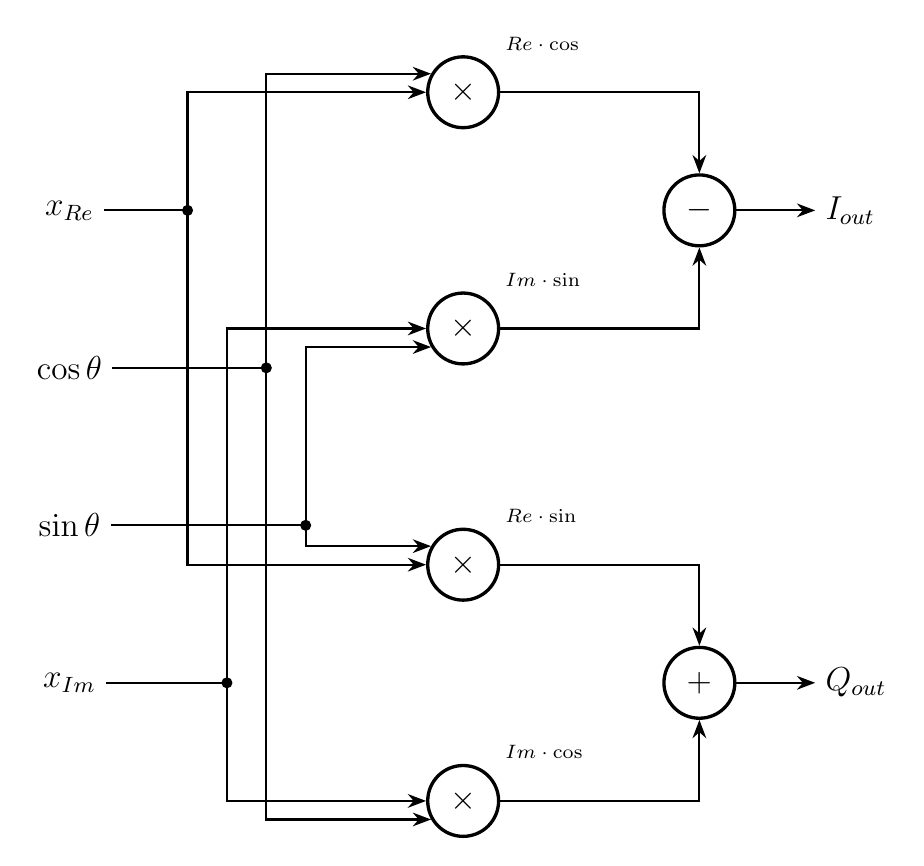
\begin{tikzpicture}[
    node distance=1.2cm and 2.5cm,
    >=Stealth,
    thick,
    font=\sffamily\large
]

% ---------------------------------------------------------
% Styles
% ---------------------------------------------------------
\tikzset{
    op_node/.style={
        circle, draw=black, very thick, minimum size=0.9cm, fill=white
    },
    io_node/.style={
        font=\bfseries\large
    },
    dot/.style={
        circle, fill=black, inner sep=0pt, minimum size=4pt
    }
}

% ---------------------------------------------------------
% 1. Multipliers (The Column Backbone)
% ---------------------------------------------------------
\node[op_node] (Mult1) at (0, 4.5) {$\times$};
\node[op_node] (Mult2) at (0, 1.5) {$\times$};
\node[op_node] (Mult3) at (0, -1.5) {$\times$};
\node[op_node] (Mult4) at (0, -4.5) {$\times$};

% Labels
\node[above right=0.1cm of Mult1, font=\scriptsize] {$Re \cdot \cos$};
\node[above right=0.1cm of Mult2, font=\scriptsize] {$Im \cdot \sin$};
\node[above right=0.1cm of Mult3, font=\scriptsize] {$Re \cdot \sin$};
\node[above right=0.1cm of Mult4, font=\scriptsize] {$Im \cdot \cos$};

% ---------------------------------------------------------
% 2. Inputs (Far Left)
% ---------------------------------------------------------
\node[io_node] (InRe)  at (-5, 3.0) {$x_{Re}$};
\node[io_node] (InCos) at (-5, 1.0) {$\cos \theta$};
\node[io_node] (InSin) at (-5, -1.0) {$\sin \theta$};
\node[io_node] (InIm)  at (-5, -3.0) {$x_{Im}$};

% ---------------------------------------------------------
% 3. Orthogonal Wiring
% ---------------------------------------------------------
% Re -> Mult1 and Mult3
\draw (InRe) -- (-3.5, 3.0) coordinate (SplitRe);
\node[dot] at (SplitRe) {};
\draw[->] (SplitRe) |- (Mult1.west);
\draw[->] (SplitRe) |- (Mult3.west);

% Im -> Mult2 and Mult4
\draw (InIm) -- (-3.0, -3.0) coordinate (SplitIm);
\node[dot] at (SplitIm) {};
\draw[->] (SplitIm) |- (Mult2.west);
\draw[->] (SplitIm) |- (Mult4.west);

% Cos -> Mult1 and Mult4
\draw (InCos) -- (-2.5, 1.0) coordinate (SplitCos);
\node[dot] at (SplitCos) {};
\draw[->] (SplitCos) |- (Mult1.150);
\draw[->] (SplitCos) |- (Mult4.210);

% Sin -> Mult2 and Mult3
\draw (InSin) -- (-2.0, -1.0) coordinate (SplitSin);
\node[dot] at (SplitSin) {};
\draw[->] (SplitSin) |- (Mult2.210);
\draw[->] (SplitSin) |- (Mult3.150);

% ---------------------------------------------------------
% 4. Output Stage
% ---------------------------------------------------------
% Subtractor
\node[op_node] (Sub) at (3, 3.0) {$-$};
% Adder
\node[op_node] (Add) at (3, -3.0) {$+$};

\draw[->] (Mult1) -| (Sub.north);
\draw[->] (Mult2) -| (Sub.south);
\draw[->] (Mult3) -| (Add.north);
\draw[->] (Mult4) -| (Add.south);

% ---------------------------------------------------------
% 5. Final Outputs
% ---------------------------------------------------------
\node[io_node, right=1.0cm of Sub] (OutI) {$I_{out}$};
\node[io_node, right=1.0cm of Add] (OutQ) {$Q_{out}$};

\draw[->] (Sub) -- (OutI);
\draw[->] (Add) -- (OutQ);

\end{tikzpicture}%
}

\vspace{5mm}
\begin{align*}
    I_{out} &= (x_{Re} \cdot \cos\theta) - (x_{Im} \cdot \sin\theta) \\
    Q_{out} &= (x_{Re} \cdot \sin\theta) + (x_{Im} \cdot \cos\theta)
\end{align*}

\noindent\textit{All four products computed in parallel (64-bit). Result truncated to $[47\!:\!16]$ (Q16.16). Enable gate provides sample-and-hold behavior.}

\caption{Complex\_Mult\_Output block -- complex multiplication with orthogonal signal routing.}
\label{fig:complex_mult}
\end{figure}


\end{document}
